\documentclass [11pt,twoside]{article}
\usepackage[utf8]{inputenc}
\usepackage[T1]{fontenc}


%Page margins, header and footer positions
\usepackage{geometry}
 \geometry{
 a4paper,
 total={210mm,297mm},
 left=25mm,
 right=25mm,
 top=30mm,
 bottom=25mm,
 headsep=7mm}

\interfootnotelinepenalty=10000

%To display filling dots in the TOC for all entries
\usepackage[titles]{tocloft}
\renewcommand{\cftsecleader}{\cftdotfill{\cftdotsep}}

%Define new header and footer style
\usepackage{fancyhdr}

\pagestyle{fancy}
\fancyhf{}
\lhead{\color{Gray}{\small{Travlendar+ project by YOUR NAMES}}}
\lfoot{\textcolor{Gray}{\small{Copyright © 2017, YOUR NAMES – All rights reserved}}}
\rfoot{\textcolor{Gray}{\thepage}}
\renewcommand{\headrulewidth}{0pt}

%PACKAGES
\usepackage{wasysym}
\usepackage{pifont}

\newcommand{\supported}{\ding{52}\xspace}
\newcommand{\unsupported}{\ding{55}\xspace}
\newcommand{\partsupported}{\textcolor{black!40}{\ding{52}}\xspace}
\newcommand{\lowsupported}{\textcolor{black!20}{\ding{52}}\xspace}
\newcommand{\unknowsupported}{\textbf{?}\xspace}

%Font: Times
\usepackage{times}
%Change monospaced font
\renewcommand{\ttdefault}{lmtt}

%tables
\usepackage{tabu}
\usepackage{tabularx}
\usepackage{ltablex}
\usepackage{longtable}
\usepackage{float} % To allow the use of H modifier in long tables

%landscape mode
\usepackage{pdflscape}
\usepackage{rotating}
\usepackage{caption}

%make landscape mode be sensitive to even and odd pages
%start
\def\myrotate{\ifodd\c@page\else-\fi 90}
\makeatletter
\global\let\orig@begin@landscape=\landscape%
\global\let\orig@end@landscape=\endlandscape%
\gdef\@true{1}
\gdef\@false{0}
\gdef\landscape{%
    \global\let\within@landscape=\@true%
    \orig@begin@landscape%
}%
\gdef\endlandscape{%
    \orig@end@landscape%
    \global\let\within@landscape=\@false%
}%
\@ifpackageloaded{pdflscape}{%
    \gdef\pdf@landscape@rotate{\PLS@Rotate}%
}{
    \gdef\pdf@landscape@rotate#1{}%
}
\let\latex@outputpage\@outputpage
\def\@outputpage{
    \ifx\within@landscape\@true%
        \if@twoside%
            \ifodd\c@page%
                \gdef\LS@rot{\setbox\@outputbox\vbox{%
                    \pdf@landscape@rotate{-90}%
                    \hbox{\rotatebox{90}{\hbox{\rotatebox{180}{\box\@outputbox}}}}}%
                }%
            \else%
                \gdef\LS@rot{\setbox\@outputbox\vbox{%
                    \pdf@landscape@rotate{+90}%
                    \hbox{\rotatebox{90}{\hbox{\rotatebox{0}{\box\@outputbox}}}}}%
                }%
            \fi%
        \else%
            \gdef\LS@rot{\setbox\@outputbox\vbox{%
                \pdf@landscape@rotate{+90}%
                \hbox{\rotatebox{90}{\hbox{\rotatebox{0}{\box\@outputbox}}}}}%
            }%
        \fi%
    \fi%
    \latex@outputpage%
}
\makeatother
%end

%graphics
\usepackage{graphicx}
\usepackage[dvipsnames, table]{xcolor}
%If you upload images from PC, you need to insert code for the path here (different for Windows and Unix OS)

%References
%\usepackage{xpatch}
%\usepackage[backend=biber, style=numeric, citestyle=numeric, sorting=none]{biblatex}
%\addbibresource{main.bib}


%Other
\usepackage{ifthen}
\usepackage{xspace}
\usepackage{enumitem}
\usepackage{amssymb}
\usepackage[pdftex, colorlinks]{hyperref}

% \hypersetup{
%     linkcolor=blue,
%     filecolor=magenta,
%     urlcolor=cyan,
%     }

\newcommand{\comment}[1]{{\color{Red}$\blacktriangleright$ Comment: #1 $\blacktriangleleft$}}


% Some utilities\ldots
\usepackage{soul}
\usepackage{tikz}

\usetikzlibrary{calc}
\usetikzlibrary{decorations.pathmorphing}


\makeatletter

\newcommand{\defhighlighter}[3][]{%
  \tikzset{every highlighter/.style={color=#2, fill opacity=#3, #1}}%
}

\defhighlighter{yellow}{.5}

\newcommand{\highlight@DoHighlight}{
  \fill [ decoration = {random steps, amplitude=1pt, segment length=15pt}
        , outer sep = -15pt, inner sep = 0pt, decorate
       , every highlighter, this highlighter ]
        ($(begin highlight)+(0,8pt)$) rectangle ($(end highlight)+(0,-3pt)$) ;
}

\newcommand{\highlight@BeginHighlight}{
  \coordinate (begin highlight) at (0,0) ;
}

\newcommand{\highlight@EndHighlight}{
  \coordinate (end highlight) at (0,0) ;
}

\newdimen\highlight@previous
\newdimen\highlight@current

\DeclareRobustCommand*\highlight[1][]{%
  \tikzset{this highlighter/.style={#1}}%
  \SOUL@setup
  %
  \def\SOUL@preamble{%
    \begin{tikzpicture}[overlay, remember picture]
      \highlight@BeginHighlight
      \highlight@EndHighlight
    \end{tikzpicture}%
  }%
  %
  \def\SOUL@postamble{%
    \begin{tikzpicture}[overlay, remember picture]
      \highlight@EndHighlight
      \highlight@DoHighlight
    \end{tikzpicture}%
  }%
  %
  \def\SOUL@everyhyphen{%
    \discretionary{%
      \SOUL@setkern\SOUL@hyphkern
      \SOUL@sethyphenchar
      \tikz[overlay, remember picture] \highlight@EndHighlight ;%
    }{%
    }{%
      \SOUL@setkern\SOUL@charkern
    }%
  }%
  %
  \def\SOUL@everyexhyphen##1{%
    \SOUL@setkern\SOUL@hyphkern
    \hbox{##1}%
    \discretionary{%
      \tikz[overlay, remember picture] \highlight@EndHighlight ;%
    }{%
    }{%
      \SOUL@setkern\SOUL@charkern
    }%
  }%
  %
  \def\SOUL@everysyllable{%
    \begin{tikzpicture}[overlay, remember picture]
      \path let \p0 = (begin highlight), \p1 = (0,0) in \pgfextra
        \global\highlight@previous=\y0
        \global\highlight@current =\y1
      \endpgfextra (0,0) ;
      \ifdim\highlight@current < \highlight@previous
        \highlight@DoHighlight
        \highlight@BeginHighlight
      \fi
    \end{tikzpicture}%
    \the\SOUL@syllable
    \tikz[overlay, remember picture] \highlight@EndHighlight ;%
  }%
  \SOUL@
}

\makeatother


% Common abbrev. are set as commands to ensure proper spacing after the dot
\RequirePackage{xspace}
\newcommand{\ie}{i.e.\@\xspace}
\newcommand{\aka}{a.k.a.\@\xspace}
\newcommand{\Ie}{I.e.\@\xspace}
\newcommand{\cf}{cf.\@\xspace}
\newcommand{\Cf}{Cf.\@\xspace}
\newcommand{\eg}{e.g.\@\xspace}
\newcommand{\Eg}{E.g.\@\xspace}
\newcommand{\etal}{et al.\@\xspace}
\newcommand{\etc}{etc.\@\xspace}
\newcommand{\wrt}{w.r.t.\@\xspace}
\newcommand{\Wrt}{W.r.t.\@\xspace}

\date{}

\begin{document}

%TITLE PAGE

\begin{titlepage}


%LOGO

% {\begin{table}[t!]
% \centering
% \begin{tabu} to \textwidth { X[1.3,r,p] X[1.7,l,p] }
% \textcolor{Blue}
% {\textbf{\small{}}} & 
\includegraphics[scale=0.5]{Images/PolimiLogo}
% \end{tabu}
% \end{table}}~\\ [7cm]

\begin{tikzpicture}[remember picture,overlay]
    \node [fill, rectangle, top color={myblue!30}, bottom color=white, anchor=north, minimum width=\paperwidth, minimum height=\paperheight] (box) at (current page.north){};
  \end{tikzpicture}

\begin{figure}[H]
	\centering
    
\includegraphics[width=\textwidth]{Images/PolimiLogo}
\end{figure}

\vfill
\vfill
%TITLE 

% \begin{flushleft}
\begin{center}
%Replace the text string with your title
% \textcolor{Blue}{\textbf{\Huge{Requirement Analysis\\ and \\Specification Document}}}
% \textcolor{myblue}{\textit{\textline[t]{Requirement Analysis}{\&}{Specification Document}}}
\textcolor{myblue}{\textit{\Huge{\textbf{Design Document}}}}
\end{center}
% \end{flushleft}



% \begin{figure}[H]
% 	\centering
%     
\includegraphics[width=0.3\textwidth]{Images/logo.pdf}
% \end{figure}

% \begin{center}
%     \textcolor{myblue}{\Huge{\textbf{DREAM}}}
% \end{center}

\vfill

\begin{center}
    \begin{adjustbox}{width=0.4\textwidth}
        \begin{tikzpicture}
        \node [circle, minimum width = 7cm,
            path picture = {
                \node [] at (path picture bounding box.center) {
                
\includegraphics[scale=0.12]{Images/logo/logo.jpg}};
                \node [] at (path picture bounding box.center) {{
                \transparent{0.8}
\includegraphics[scale=0.4]{Images/logo/onu.png}}};
            }] {};
        % \path 
            % [rotate=125,postaction={decoration={text along path,text={|\huge\bfseries|\ DREAM - Data-dRiven prEdictive fArMing -},
            %   text align=fit to path,reverse path}, decorate}]
            %  circle[radius=3cm] ; 
        \path 
            [rotate=232,postaction={decoration={text along path,text={|\huge\bfseries|\ Data-dRiven prEdictive fArMing {\Large\textbullet} {\myrotate{M}}{\myrotate{A}}{\myrotate{E}}{\myrotate{R}}{\myrotate{D}} {\Large\textbullet}}, text align=fit to path,reverse path}, decorate}]
            circle[radius=4cm];
        \end{tikzpicture}
    \end{adjustbox}
\end{center}

\vfill
\end{titlepage}


%Define deliverable specific info
%Replace cell contents where needed
% \begin{table}[h!]
% \begin{tabu} to \textwidth { X[0.2,r,p] X[0.7,l,p] }
% \hline

% \textbf{Deliverable:} & RASD\\
% \textbf{Title:} & Requirement Analysis and Verification Document \\
% \textbf{Authors:} & Leonardo Gori, Marco Romanini, Yui Watanabe \\
% \textbf{Version:} & 1.0 \\ 
% \textbf{Date:} & 31-January-2016 \\
% \textbf{Download page:} & https://github.com/MarcoRomanini/GoriRomaniniWatanabe \\
% \textbf{Copyright:} & Copyright © 2017, Leonardo Gori, Marco Romanini, Yui Watanabe – All rights reserved \\
% \hline
% \end{tabu}
% \end{table}


\begin{table}[H]
    \setlength\arrayrulewidth{1pt}
    \centering
    \rowcolors{1}{myblue!25}{white}
    \begin{tabular}{rl}
        \hline
        \textbf{Deliverable:} & DD\\
        \textbf{Title:} & Design Document \\
        \textbf{Authors:} & Leonardo Gori, Marco Romanini, Yui Watanabe \\
        \textbf{Version:} & 1.0 \\ 
        \textbf{Date:} & \today \\
        \textbf{Download page:} & \url{https://github.com/MarcoRomanini/GoriRomaniniWatanabe} \\
        \textbf{Copyright:} & Copyright © 2021, Leonardo Gori, Marco Romanini, Yui Watanabe – All rights reserved \\
        \hline
    \end{tabular}
\end{table}

\setcounter{page}{2}


%------------------------------------------------------------------------------------------------------------------------------------------------
\newpage
\addcontentsline{toc}{section}{Table of Contents}
\tableofcontents
\newpage
\addcontentsline{toc}{section}{List of Figures}
\listoffigures
\addcontentsline{toc}{section}{List of Tables}
\listoftables

%------------------------------------------------------------------------------------------------------------------------------------------------
\clearpage
{\color{Blue}{\section{\label{sect:introduction}Introduction}}}

This document has been prepared to help you approaching Latex as a formatting tool for your Travlendar+ deliverables. This document suggests you a possible style and format for your deliverables and contains information about basic formatting commands in Latex. A good guide to Latex is available here \href{https://tobi.oetiker.ch/lshort/lshort.pdf}{https://tobi.oetiker.ch/lshort/lshort.pdf}, but you can find many other good references on the web. 

Writing in Latex means writing textual files having a \texttt{.tex} extension and exploiting the Latex markup commands for formatting purposes. Your files then need to be compiled using the Latex compiler. Similarly to programming languages, you can find many editors that help you writing and compiling your latex code. Here \href{https://beebom.com/best-latex-editors/}{https://beebom.com/best-latex-editors/} you have a short oviewview of some of them. Feel free to choose the one you like.  

Include a subsection for each of the following items\footnote{By the way, what follows is the structure of an itemized list in Latex.}:
\begin{itemize}
\item
Purpose: here we include the goals of the project
\item
Scope: here we include an analysis of the world and of the shared phenomena
\item
Definitions, Acronyms, Abbreviations
\item
Revision history
\item
Reference Documents 
\item
Document Structure
\end{itemize}
Below you see how to define the header for a subsection.
\subsection{Scope}
... Here you see a subsubsection
\subsubsection{World Phenomena}
%what you write here is a comment that is not shown in the final text
In this section \ldots

\begin{figure}[H]
	\centering
    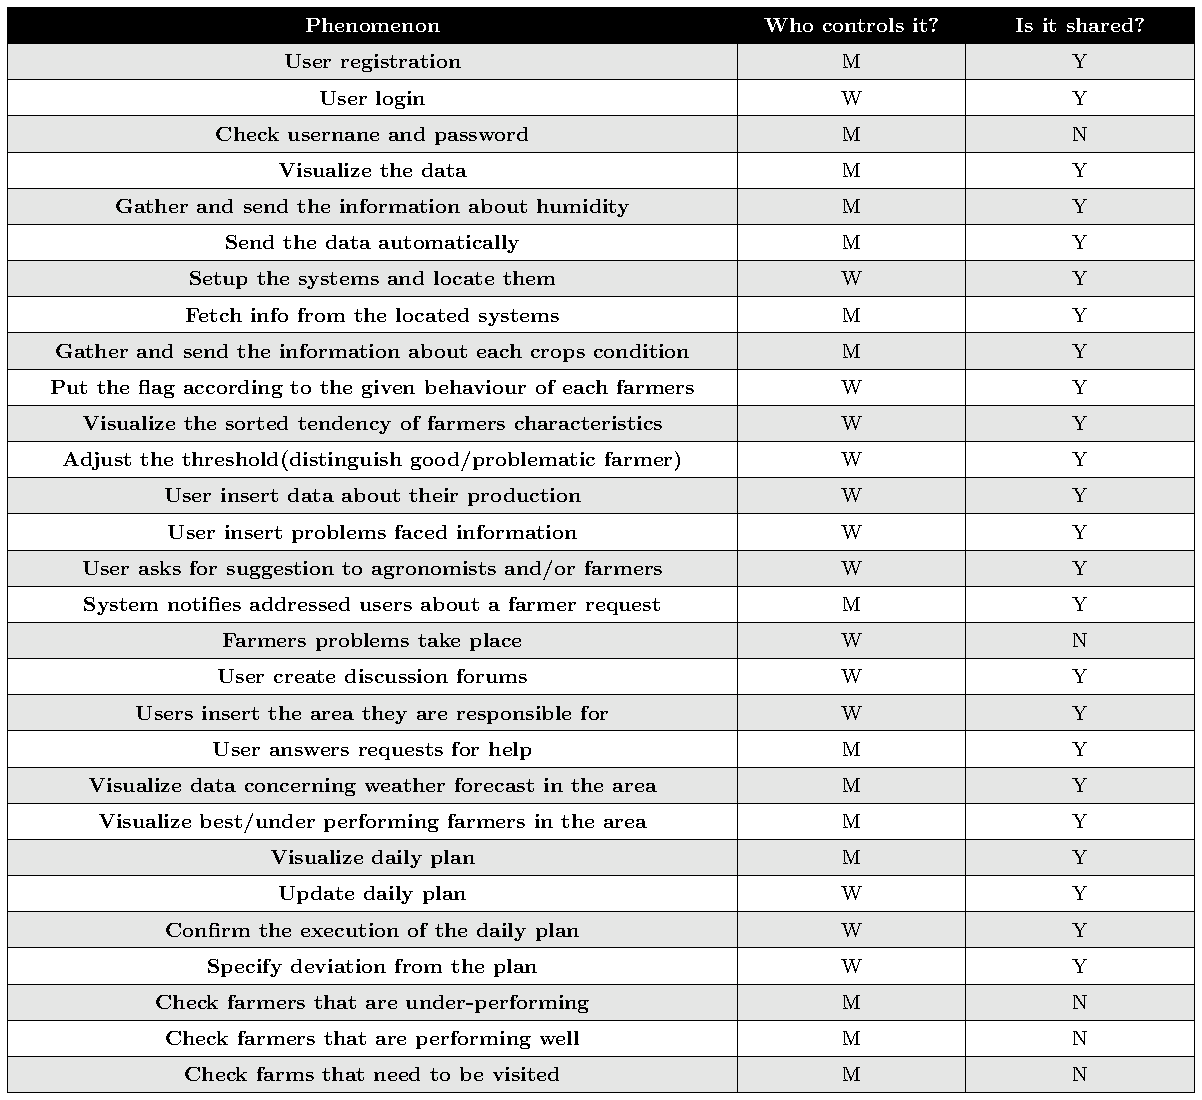
\includegraphics[page=1, width=\textwidth]{Tikz_stuff/Phenomena _table_external_project.pdf}
	\caption{\label{tab:phenomena}Phenomena table}
\end{figure}

% TODO Define verbs conventions of ISO/IEEE
% TODO Requirements should be ranked for importance or stability (from Hans Van Vliet book)

%------------------------------------------------------------------------------------------------------------------------------------------------
\clearpage
{\color{Blue}{\section{\label{sect:architectural_design}Architectural design}}}


% ############### 2) ARCHITECTURAL DESIGN ####################

% 2.1
\subsection{Overview}
\label{sec:overview}

% ############### PRODUCT PERSPECTIVE ####################à
\subsection{Product perspective}
\hyperref[tab:acronymsTable]{DREAM} is a functional multi-user software platform whose purpose is to provide functionalities described in section \ref{sect:product_functions}. The system will be composed by a series of software and hardware interfaces that interact in such a way to let users manipulate shared data. It also will exploit some graphical interface packages in order to be user friendly and easy to use.
This product is designed to run on a wide variety of machines, including operating systems Mac OS, Windows, Linux, Android and iOS. 

\begin{figure}[H]
	\centering
    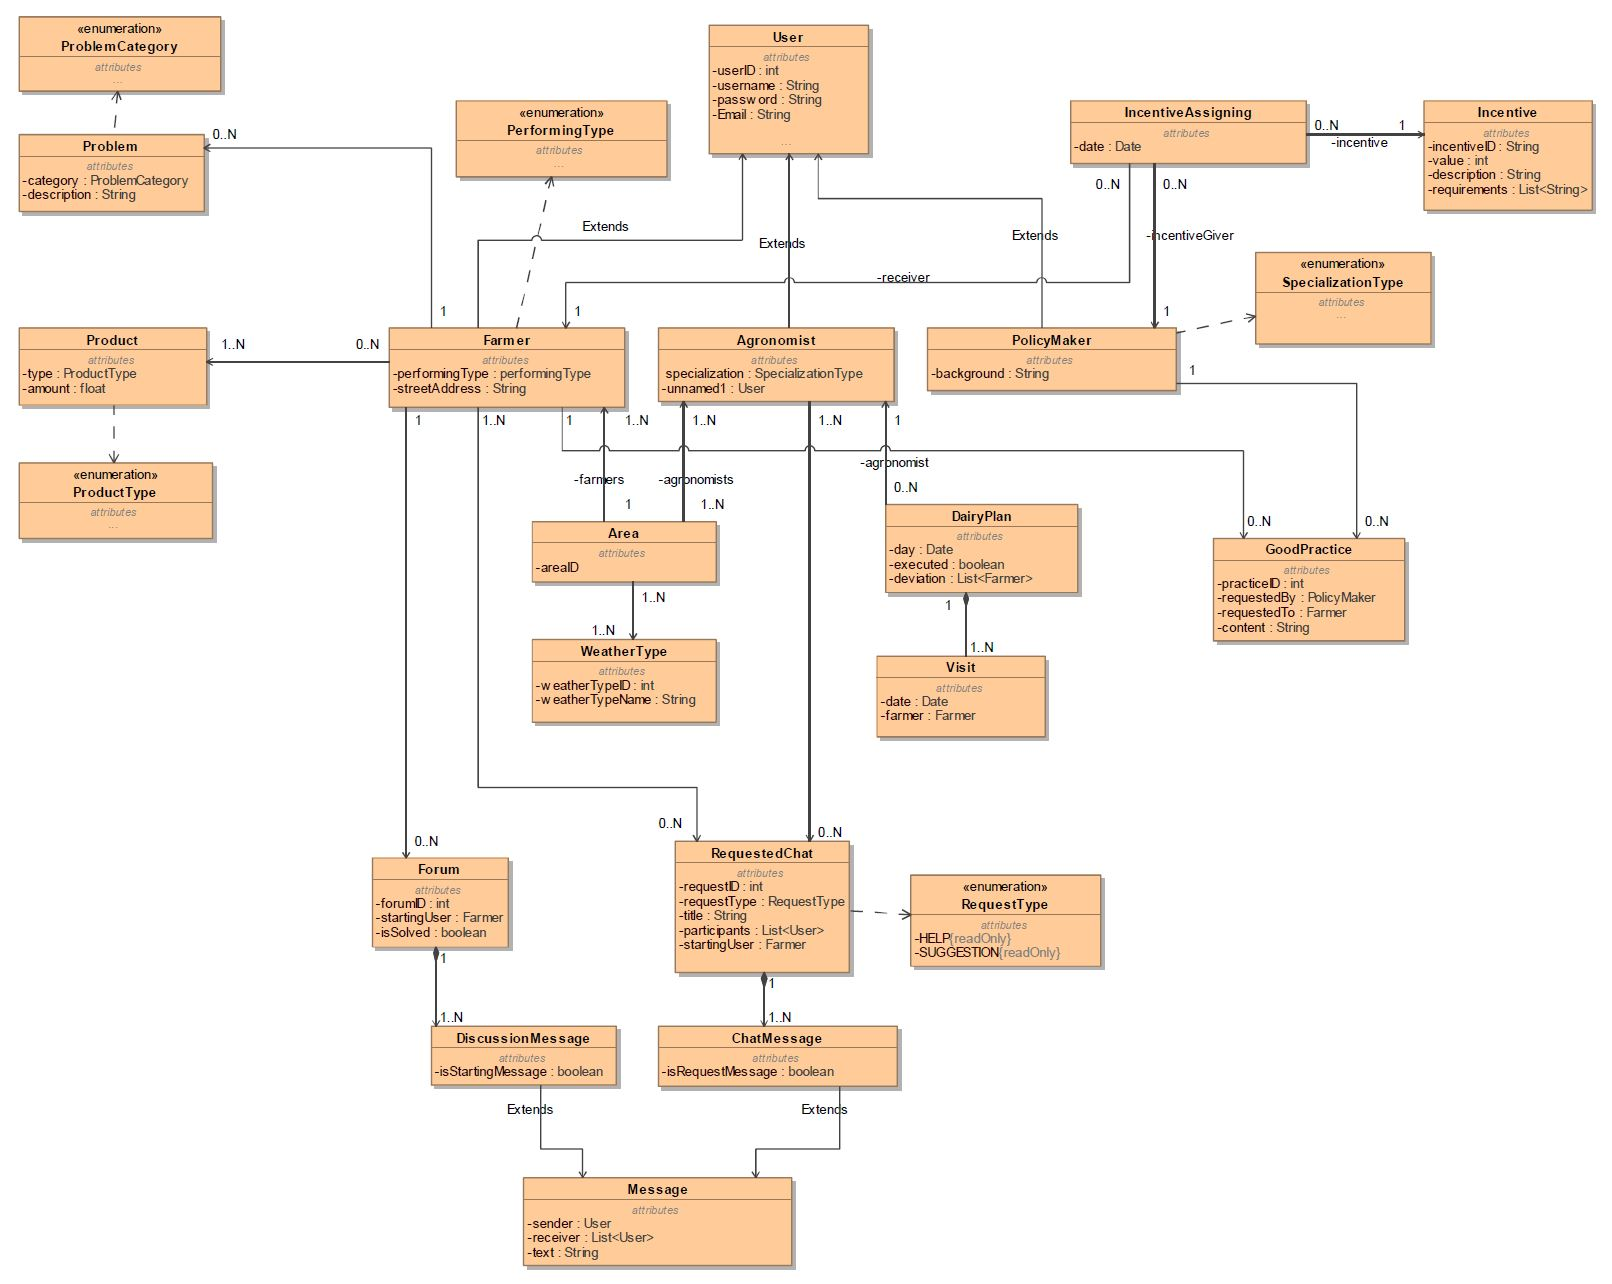
\includegraphics[page=1, width=\textwidth]{Images/uml.JPG}
	\caption{\label{fig:uml_class_diagram}High level UML diagram}
\end{figure}


\subsubsection*{UML description}
\begin{center}
    \setlength\arrayrulewidth{1pt}
    \rowcolors{2}{white}{myblue!25}
    \begin{longtable}{|c|m{0.7\textwidth}|}
            
            \hline
            \rowcolor{myblue}\color{white}Class & \color{white}Description \\
            \hline
            
            \textsc{User}  &    This class represents the people registered to the system, with their credentials  \\
            \hline
            \textsc{Farmer}     &   This class represents the farmers, with their performing type and their street address (information useful to agronomists) \\
            \hline
            \textsc{Agronomist}  &    This class represents the agronomists, with their specialization type \\
            \hline
            \textsc{PolicyMaker}  &    This class represents the policy makers, with their background (e.g., India’s government, Telangana’s government, United Nations, etc)  \\
            \hline
            \textsc{Area}  &    This class represents the areas in which Telangana has been divided for the management of this system. Areas can be the 33 districts in which Telangana is formally divided, but a different subdivision criteria can be used  \\
            \hline
            \textsc{WeatherType}  &    This class represents some characteristics of the area regarding weather aspects (e.g., humidity, rainfall frequency, average temperature, etc)  \\
            \hline
            \textsc{Forum}  &    This class represents the discussion forums that farmers can use to communicate with each other, to get information and to exchange ideas. Only farmers can write in forums  \\
            \hline
            \textsc{RequestChat}  &    This class represents the requests that farmers can send to agronomists and to other farmers. Requests can be for help or for suggestions. A request is modelled as a chat where the participants are selected by the farmer that makes the request. A request always has at least one agronomist as a participant \\
            \hline
            \textsc{Message}  &    This class represents the messages exchanged in forums and chats across the platform, with their sender, receivers and text  \\
            \hline
            \textsc{DiscussionMessage}  &    This class represents the messages belonging to forums. For every forum there is only one starting message, while all the other messages are considered as replies to that message  \\
            \hline
            \textsc{ChatMessage}  &    This class represents the messages belonging to request chats. For every request there is only one message of type “request ”(the first message), while all the other messages are considered as “reply”. Every chat message is delivered to all the participants of that chat (excluding the sender, of course)  \\
            \hline
            \textsc{DailyPlan}  &    This class represents the daily plans of the agronomists, with the date, the list of visits for that day and the list of unvisited farmers (once the plan has been executed)  \\
            \hline
            \textsc{Visit}  &    This class represents the visits that agronomists arrange for checking the farmers’ activity  \\
            \hline
            \textsc{Product}  &    This class represents the products that are inserted in the system by the farmers, with their type and their amount  \\
            \hline
            \textsc{Problem}  &    This class represents the problems that farmers may encounter, with their category and description  \\
            \hline
            \textsc{Incentive}  &    This class represents the incentives that are available for farmers, with their description, their value and their set of requirements. Incentives are modelled as some sort of vouchers  \\
            \hline
            \textsc{IncentiveAssigning}  &    This class represents the assignments of incentives, expressed as a mapping between “when”, “to who” and “from who” a certain incentive has been given  \\
            \hline
            \hline
            \textsc{PerformingType}  &    This enumeration represents the performance type of farmers, giving information about how good a farmer is doing (for example: well-performing, normal-performing, under-performing)  \\
            \hline
            \textsc{SpecializationType}  &    This enumeration represents the type of agronomists’ specializations \\
            \hline
            \textsc{RequestType}  &    This enumeration represents the type of requests, which can be for help or for suggestions  \\
            \hline
            \textsc{ProblemCategory}  &    This enumeration represents the type of problems that farmers can face and insert into the system  \\
            \hline
        
        \rowcolor{white}\caption{UML description table}
        \label{tab:UML_description_table}
    \end{longtable}
\end{center}


\subsubsection{User interfaces}
\label{sect:user_interfaces}
According to the assignment document, the system will interact with 3 different user classes: policy makers, farmers and agronomists. In order to be more accessible and to fulfill the user needs, the application will be supported by different devices. These users should interface to the service through electronic devices with an internet connection. Users that need to access the service will have the possibility to connect through:
\begin{itemize}
    \item an internet browser, addressing a specific web domain (such as \textit{www.dream.com}) that permits users to sign up/in a dedicated web application;
    \item a mobile application that can be installed on smartphones or tablets (both iOS and Android).
\end{itemize}


\subsubsection{Software interfaces}
In order to improve software flexibility and quality, \hyperref[tab:acronymsTable]{DREAM} will use a set of external software interfaces. Rather than providing names of real specific services, we consider reasonable referring to them as functionalities to be later defined in the design phase:
\begin{description}[font=~\normalfont\scshape]
    \item[\textbf{\textcolor{myblue}{universal logins}}] \hfill \\Login \hyperref[tab:acronymsTable]{APIs} that also provide access by using their Facebook, Twitter, or Google profile login details are good candidates in order to quickly authenticate the user while guaranteeing security.
    \item[\textbf{\textcolor{myblue}{big data manipulation}}] \hfill \\Since a wide quantity of information needs to be recorded and accessed in a distributed system fashion, \hyperref[tab:acronymsTable]{DBMS} \hyperref[tab:acronymsTable]{APIs} are necessary for data extraction performances optimization.
    \item[\textbf{\textcolor{myblue}{third party data sets access}}] \hfill \\
    The system will use open data sets to obtain information about weather forecasts, soil moisture, water irrigation, humidity and so on.
    \item[\textbf{\textcolor{myblue}{farmers evaluation}}] \hfill \\
    To evaluate the performance of farmers, the system relies on external \hyperref[tab:acronymsTable]{APIs} that use specific algorithms to understand how good a farmer is doing (positive or negative deviance).
    \item[\textbf{\textcolor{myblue}{incentives management}}] \hfill \\
    The system will rely on an external service for the definition of incentives and for their money collection by the farmers.
    \item[\textbf{\textcolor{myblue}{weather types categorization}}] \hfill \\
    To define the weather type categories of the areas, the system will use some sort of \hyperref[tab:acronymsTable]{API} to analyse areas characteristics and tendencies in order to define shared phenomena. 
    
    
\end{description}

\subsubsection{Hardware interfaces \& constraints}
DREAM system will be composed by multiple different hardware components which can be described from two points of view:
\begin{description}[font=~\normalfont\scshape]
    \item[\textbf{\textcolor{myblue}{user perspective}}] \hfill \\Since \hyperref[tab:acronymsTable]{DREAM} platform is accessed by users in a fully virtual fashion, the minimum required hardware interfaces are the ones that provides internet connection, input components, a screen to visualize \hyperref[tab:acronymsTable]{GUI} and a web browser or an application store (like smartphones, personal computers, tablets and smart TVs).
    \item[\textbf{\textcolor{myblue}{system perspective}}] \hfill \\According to the assignment, the system should be composed by hardware devices designed to gather Telangana's environment information such as soil humidity sensor and the ones responsible for the predefined water irrigation system.
\end{description}
The user hardware interfaces also represent constrains that are required in order to permit the users to interact with the systems and manipulate shared data.

\subsection{Product functions}
\label{sect:product_functions}
In this section the main functionalities of the \hyperref[tab:acronymsTable]{S2B} are presented, described and enriched with \hyperref[tab:acronymsTable]{BPMN} diagrams in order to guarantee an higher level of understanding.
\subsubsection{Sign up}
This functionality allows the user to create an account to access the platform.
Firstly he opens the sign up page and fills the information required such as email, address etc.
Then, if the inserted data is accepted, an e-mail is sent to the User asking for their verification.
Lastly, if all the steps above are done, the user is redirected to the login page.

\begin{figure}[H]
	\centering
    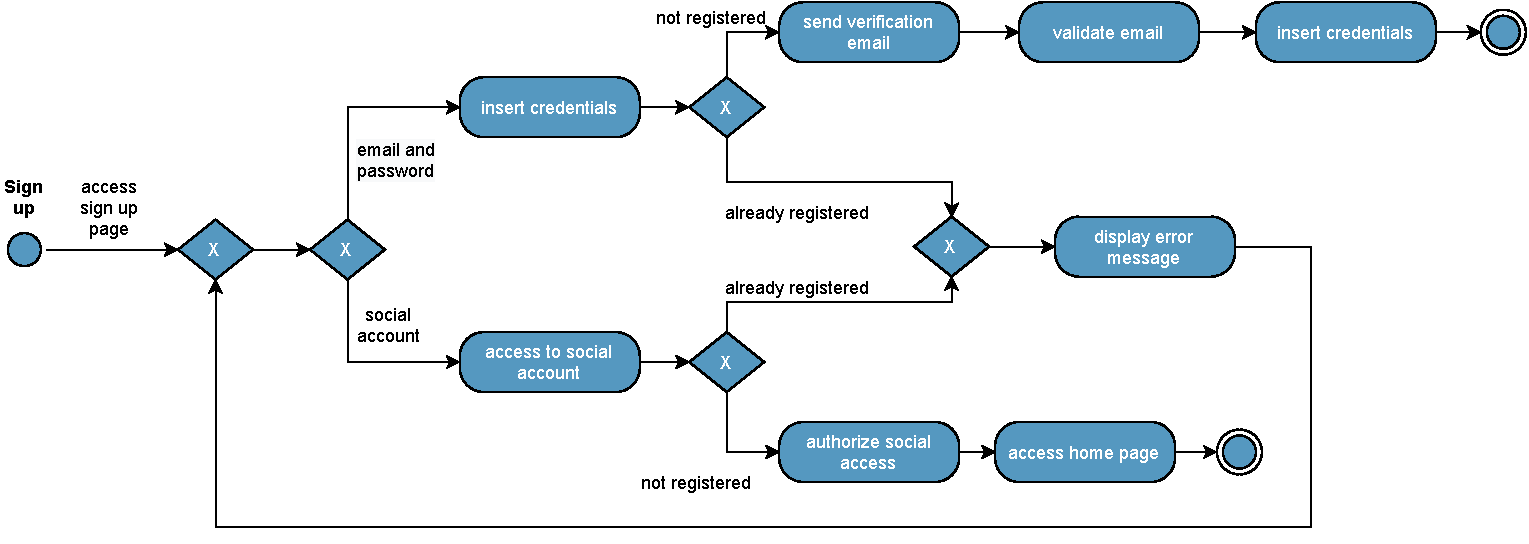
\includegraphics[width=\textwidth]{Images/BPMN/signup.pdf}
	\caption{\label{fig:bpmn_sign_up}BPMN diagram of sign Up}
\end{figure}

\subsubsection{Sharing issues to get help and suggestions}
This functionality is available for farmers and agronomists. The farmer selects the request section and the system displays the send request button; if it is clicked, all the saved contacts are shown. After selecting to whom to ask, insert the question in the text form, presses send button, then the request is sent successfully.


\begin{figure}[H]
	\centering
    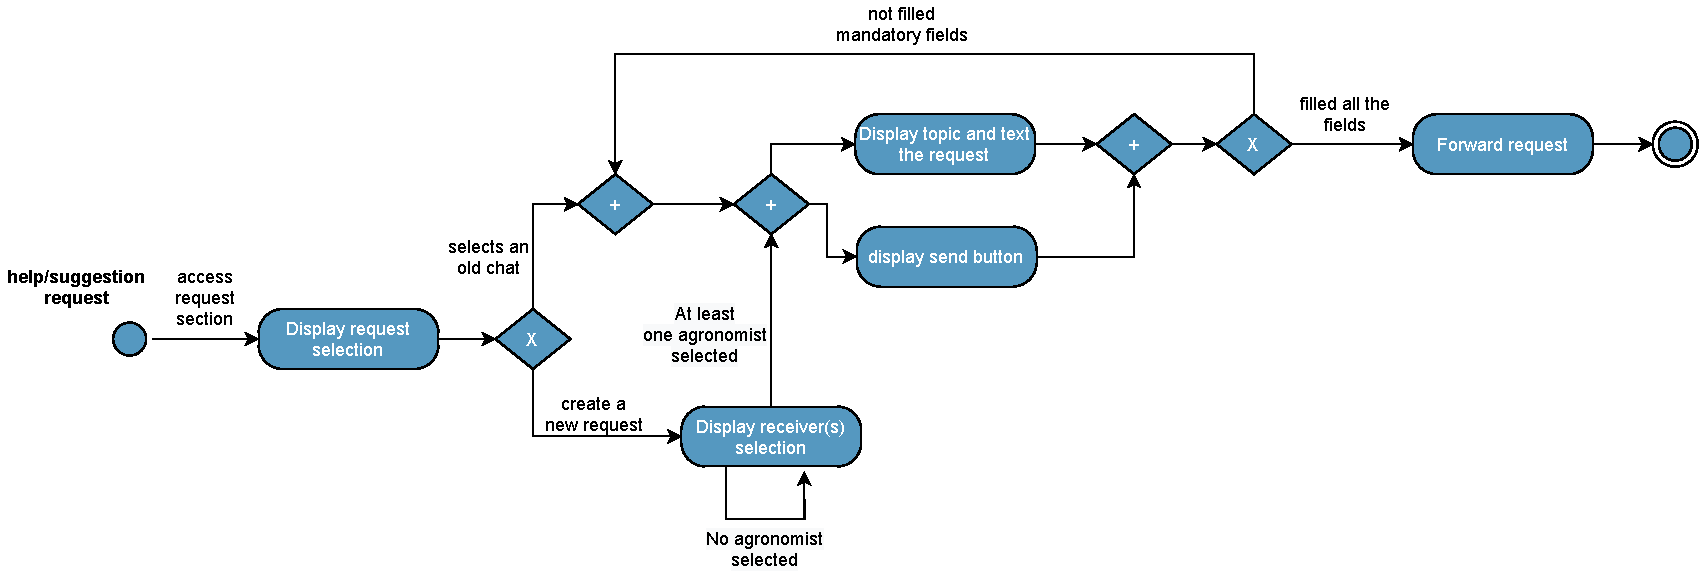
\includegraphics[width=\textwidth]{Images/BPMN/help-suggestion-request.pdf}
	\caption{\label{fig:bpmn_request}BPMN diagram of help/suggestion request}
\end{figure}


\subsubsection{Communication (among farmers) on forums}
This functionality is required for allowing farmers to exchange their opinions. The farmer accesses the forum section which presents an eventual list that contains both previous submitted forums and farmer’s forum replies. By selecting forum upload button, the system displays 
insertion form containing topic/context of the thread, title and question content. If the farmer 
inserts all the required data correctly and presses the submission button, confirmation page is shown. Lastly, by clicking confirm button the forum is generated. 

\begin{figure}[H]
	\centering
    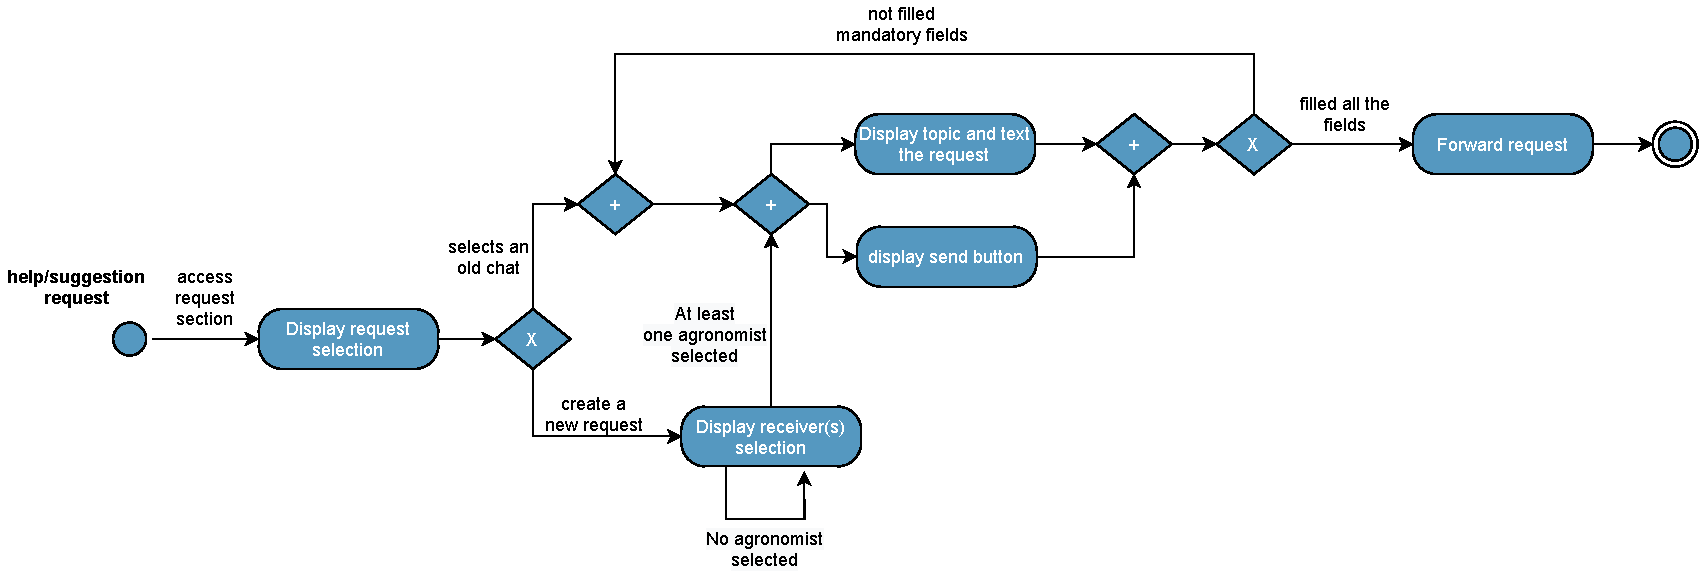
\includegraphics[width=\textwidth]{Images/BPMN/help-suggestion-request.pdf}
	\caption{\label{fig:bpmn_forum_generation}BPMN diagram of forum generation}
\end{figure}


\subsubsection{Visits to low performing farmers}
This functionality is necessary to organize the visits in order to make the schedule well-shared between an agronomist and a farmer. The agronomist goes to the daily plan section and the application displays a visualize or update button. If it is clicked, the system extracts their schedule data which is shortly expressed by a form with day-month-year and the farmers to visit.
If there is a wish to modify the plan, it is possible to modify it in a form guided by selecting the update button.

\begin{figure}[H]
	\centering
    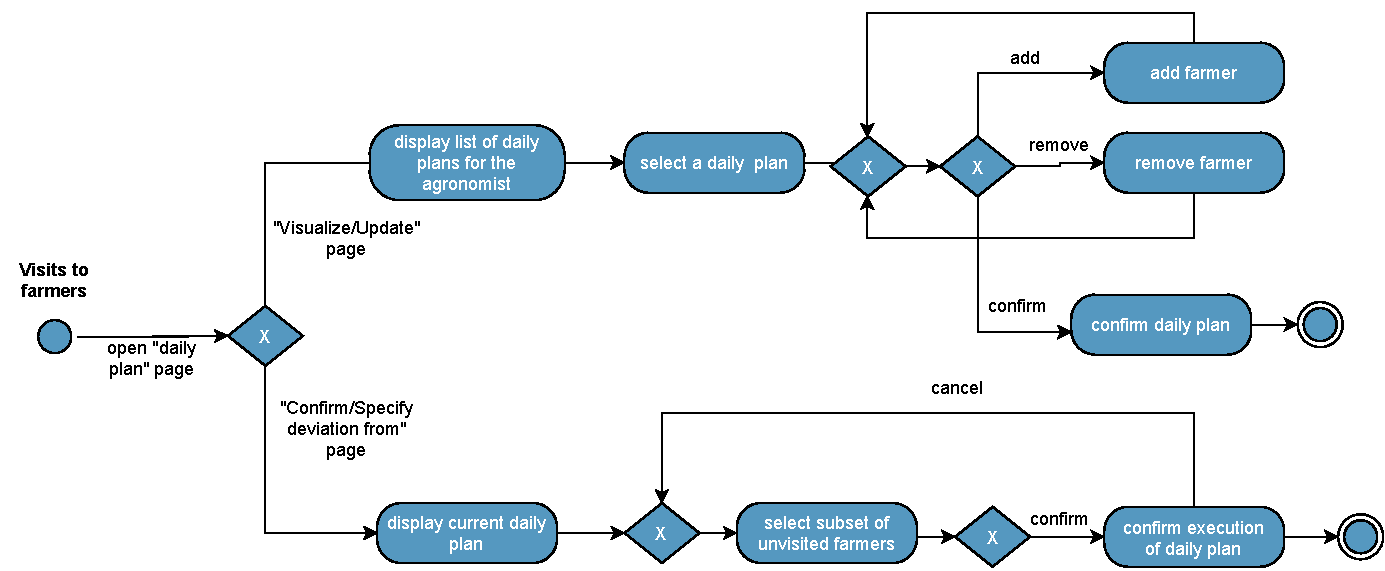
\includegraphics[width=\textwidth]{Images/BPMN/visit.pdf}
	\caption{\label{fig:bpmn_visit}BPMN diagram of visit farmers}
\end{figure}


\subsubsection{Visualize data about performance}
This functionality is used by policy makers. The policy maker clicks the farmer's performance button and the system visualize the list of farmers grouped by their production performance. If there is any interesting farmer, by selecting his/her name, the application shows the information of his/her production history.

\begin{figure}[H]
	\centering
    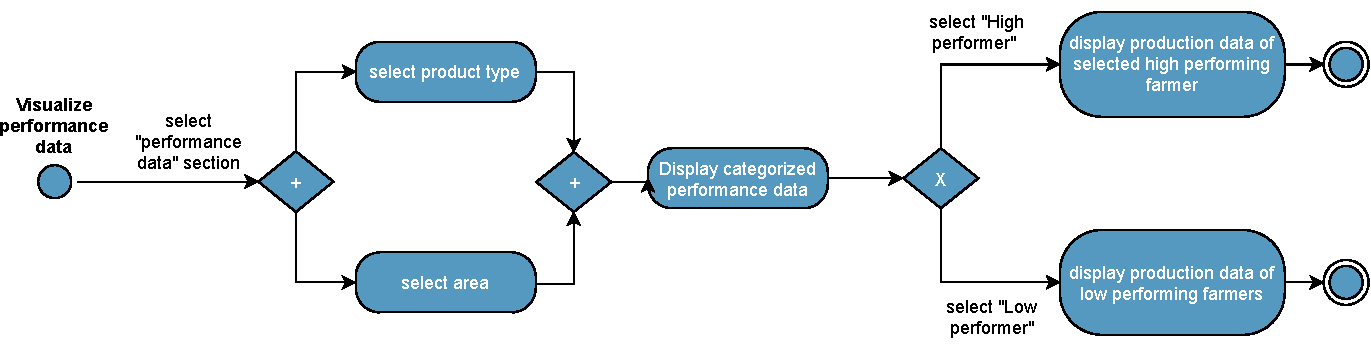
\includegraphics[width=\textwidth]{Images/BPMN/Performance.pdf}
	\caption{\label{fig:bpmn_performance}BPMN diagram of farmer performance}
\end{figure}

\subsection{Actors}
\label{sec:actors}
In this section are defined the professional figures which, according to the assignment, the system will interact with: \textbf{policy makers}, \textbf{farmers} and \textbf{agronomists}. In order to avoid redundancy, we also introduce the concept of \textbf{user} as an abstract entity that collects their common properties. As shown in figure \ref{fig:uml_class_diagram}, they inherit user's properties.
\subsubsection*{User}
It is a person who wants to use the service. In order to access the system, it has to register to the platform (the first time) and be logged in (the following times). It also requires an Internet connection to properly use the system.
\subsubsection*{Policy maker}
It is someone interested in the overall performing situation of Telangana’s farmers (e.g., Telangana’s government). It is able to surf on \hyperref[tab:acronymsTable]{DREAM}’s website. It uses the service to visualise information about well and under-performing farmers and to understand if the steering initiatives are producing significant results. We assume that those who register to the platform as policy makers are some sort of "authorized" people (for example, people working for public institutions or government) since they are allowed to actively assign incentives.
\subsubsection*{Farmer}
It is a farmer of Telangana. It is able to surf on \hyperref[tab:acronymsTable]{DREAM}’s website (or to use the smartphone application). It uses the service in order to discuss with other farmers, to send requests for help to an agronomist, to insert product information, to know when it will receive a visit from an agronomist. It takes advantage in using the system because it can receive incentives if it is well-performing or can receive help if it is under-performing.
\subsubsection*{Agronomist}
It is an agronomist of Telangana. It is able to surf on \hyperref[tab:acronymsTable]{DREAM}’s website (or to use the smartphone application). It uses the service to answer farmers' requests for help, to visualise data concerning their areas (weather forecasts, well and under-performing farmers, problems encountered by farmers), to visualise and update a daily plan to visit farms in the area, to confirm the execution or specify deviation from the daily plan.

\newpage

\subsection{Assumptions, dependencies and constraints}
\label{sec:domain_assumptions}
In this section we present the assumptions that are expected to hold in the world, the part of the environment that the machine cannot perceive nor control. The satisfaction of these so called \textbf{domain assumptions} are deeply related to the reliability of the system to behave in the expected way. If at least one of these assumptions is discovered not to be guaranteed, then the expected behaviour of the machine would allow the occurrence of an unstable state of the machine with unpredictable results.
\newline

\begin{table}[H]
    \setlength\arrayrulewidth{1pt}
    \centering
    \rowcolors{2}{white}{myblue!25}
    \begin{tabular}{|l|m{0.85\textwidth}|}
        \rowcolor{myblue}
        \hline
        \color{white}DX & \color{white}Definition \\
        \hline
        \textsc{D1}  &    Data concerning meteorological short-term and long-term forecasts is exact and reliable \\
        \hline
        \textsc{D2}     &   Information obtained by the water irrigation system is reliable \\
        \hline
        \textsc{D3}  &    Information on the humidity of soil obtained by sensors deployed on the territory is reliable\\
        \hline
        \textsc{D4}  &    Each user who wants to use the online service (web page, app) must have a device connected to Internet\\
        \hline
        \textsc{D5}  &    The user is supposed to be at least 18 years old\\
        \hline
        \textsc{D6}  &    The third party analysis about how good a farmer is doing is reliable\\
        \hline
        \textsc{D7}  &    The categorized weather types provided by a third party analysis are reliable\\
        \hline
        \textsc{D8}  &     The weather information provided by a third party is reliable \\
        \textsc{D9}  &     The third party analysis about the effectiveness of the steering initiatives is reliable \\
        \hline
        
        \hline
        \hline
        \hline
        \textsc{D10}  &    Observation of  farmers' performance is done frequently by policy makers\\
        \hline
        \textsc{D11}  &    Policy maker has enough information and knowledge to understand the proper moment to ask for good practices\\
        \hline
        \textsc{D12}  &    Outstanding high performing farmers are asked by policy makers to write their good practices periodically\\
        \hline
        \textsc{D13}  &     Incentive assignment done by policy makers is reliable \\
        \hline
        
        \hline
        \hline
        \hline
        
        \textsc{D14}  &    Information stored in the system by farmers is reliable (e.g. farmers do not insert false data about their production or their problems to look better/worse performing)\\
        \hline
        \textsc{D15}  &    When a problem occurs, farmers insert that information in the system\\
        \hline
        \textsc{D16}  &    Farmers usually interact with the system (periodic product information upload, checking for agronomist visits) \\
        \hline
        \textsc{D17}     &   When a farmer starts a forum thread, a reply will be given as soon as possible \\
        \hline
        \textsc{D18}  &    Farmer agrees on allowing the system to store information about them (location of the activity, information on production, ...)\\
        \hline
        
        
        \hline
        \hline
        \hline
    
        \textsc{D19}  &    Information inserted in the system by agronomists is reliable\\
        \hline
        \textsc{D20}  &    When an agronomist plans the visits of a daily plan, most farmers will be present\\
        \hline
        \textsc{D21}  &    Agronomists will always confirm the execution (specifying deviations, if needed) of the daily plan at the end of the same day\\
        \hline
        \textsc{D22}  &    An agronomist is responsible for several areas\\
        \hline
        
        
        
       
        
        
    \end{tabular}
    
    \caption{\label{tab:domainAssumptions}Table of domain assumptions}
    
\end{table}

\tmref{link to traceability matrix}

% 2.2
\subsection{Component view}
\label{sec:component_view}
% ############### 2.2) COMPONENT VIEW ####################
% sources:
% https://www.ibm.com/cloud/learn/microservices#toc-common-pat--cw3xiYi
% https://www.devteam.space/blog/microservice-architecture-examples-and-diagram/


In order to reduce the complexity of the \textbf{solution domain} (cfr. \cite{bruegge2013object}, \S 6.3.2), the required functionalities of the software are here decomposed by solution domain classes. A domain consists of multiple sub-domains: replaceable parts of the system with well-defined interfaces that encapsulates the state and behavior of their contained classes. Each sub-domain corresponds to a different part of the business. By decomposing the system into relatively independent subsystems, concurrent teams can work on individual subsystems with minimal communication overhead.

Some business functionalities require the aggregation of microservices functionalities (\ie for processing complex queries about farmer's information). As described in section \ref{sec:styles_patterns}, the system should make use of the CQRS pattern to fulfill the above mentioned requirement. Here we provide the internal structure that the interested microservice components should implement to achieve this task:


% (https://microservices.io/patterns/decomposition/decompose-by-subdomain.html)
\begin{figure}[H]
	\centering
    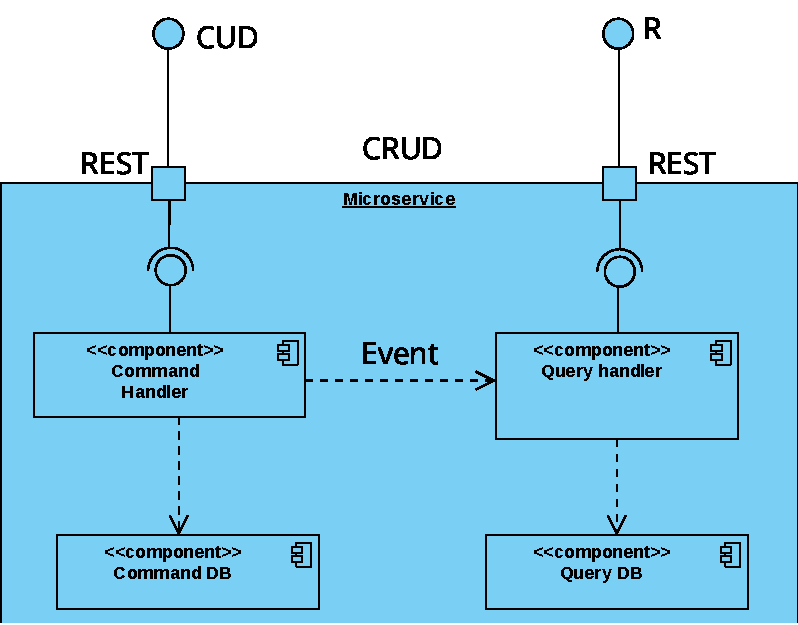
\includegraphics[ width=0.5\textwidth]{Images/CRUD_microservice.pdf}
	\caption{\label{fig:CRUD_microservice}CQRS-based microservice}
\end{figure}


In a CQRS-based service (ref.\cite{richardson2018microservices}, \S7.2.2), the command-side domain module handles CRUD operations and is mapped to its own database. It handles simple queries, such as non join, primary key-based queries. The command side publishes domain events whenever its data changes. These events might be published using event sourcing.

A separate query module handles simple queries. It’s much simpler than the command side because it’s not responsible for implementing the business rules. The query side uses whatever kind of database makes sense for the queries that it must support. The query side has event handlers that subscribe to domain events and update
the database.

The overall component diagram is shown below:

% \begin{figure}[H]
%     \makebox[\textwidth]{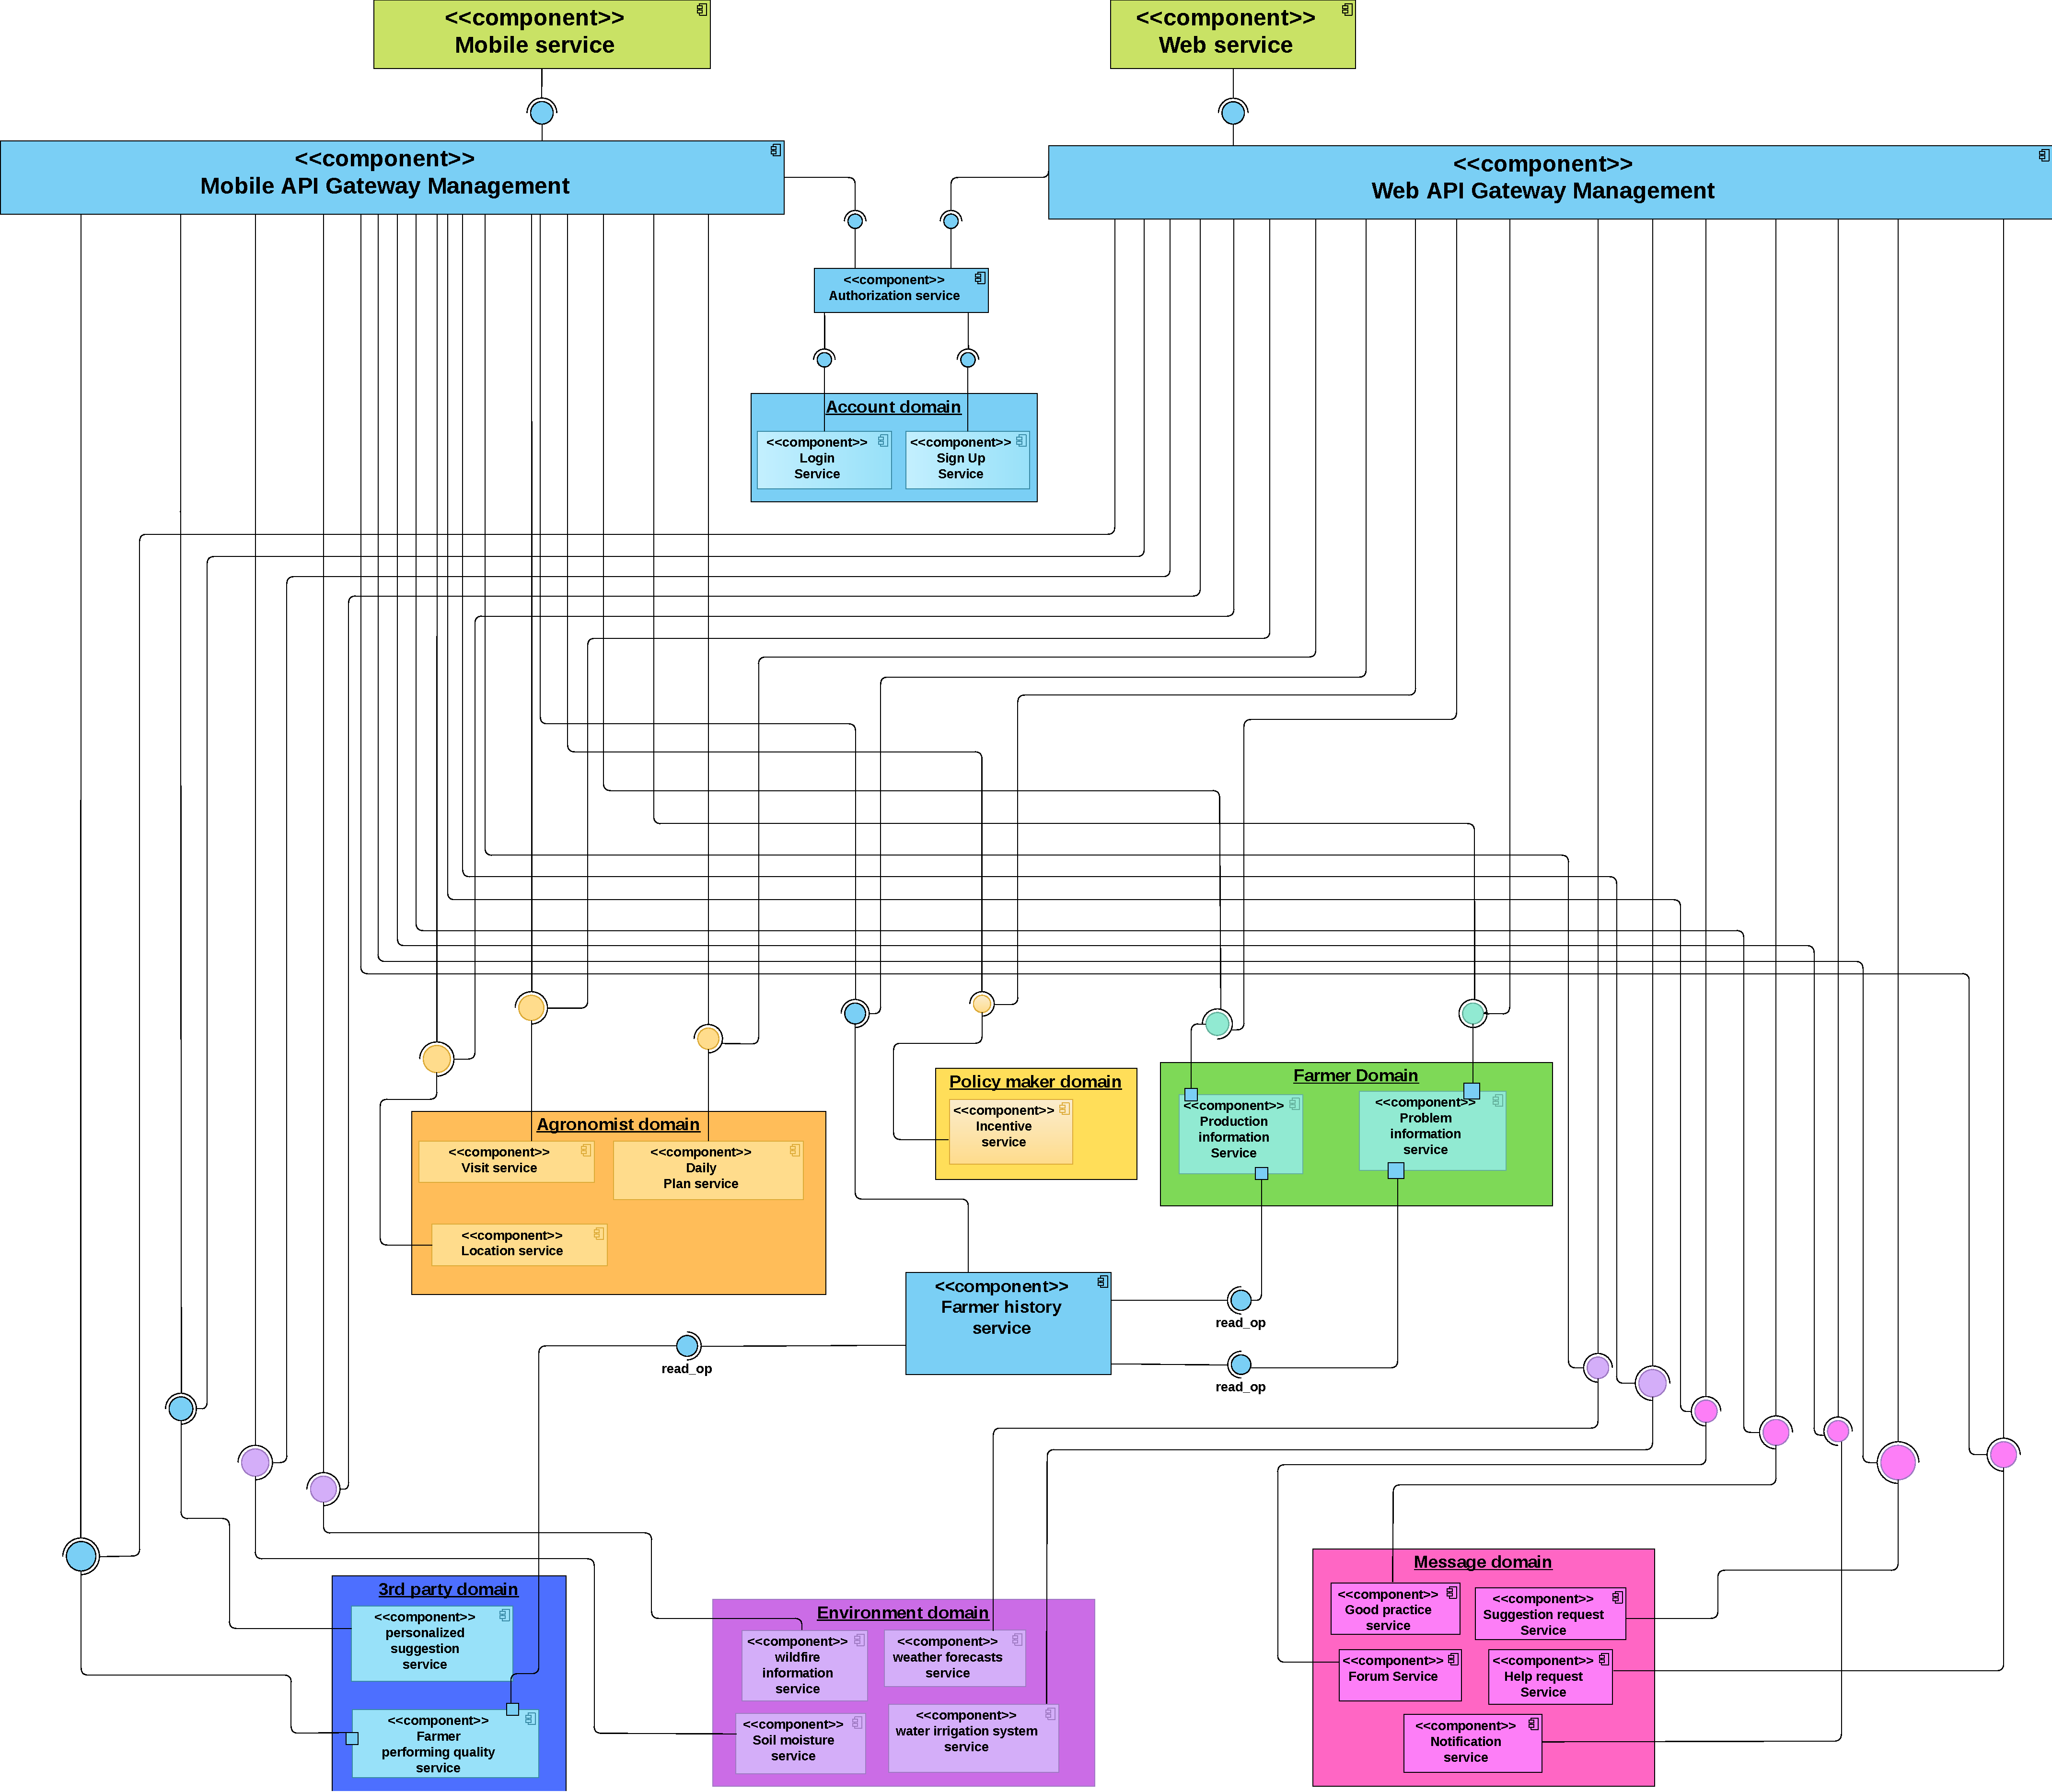
\includegraphics[width=0.99\textheight, angle=90]{Images/Component Diagram2.pdf}}
%     \caption{\label{fig:component_diagram_rotated}comp diagram}
% \end{figure}

\begin{figure}[H]
    \makebox[\textwidth]{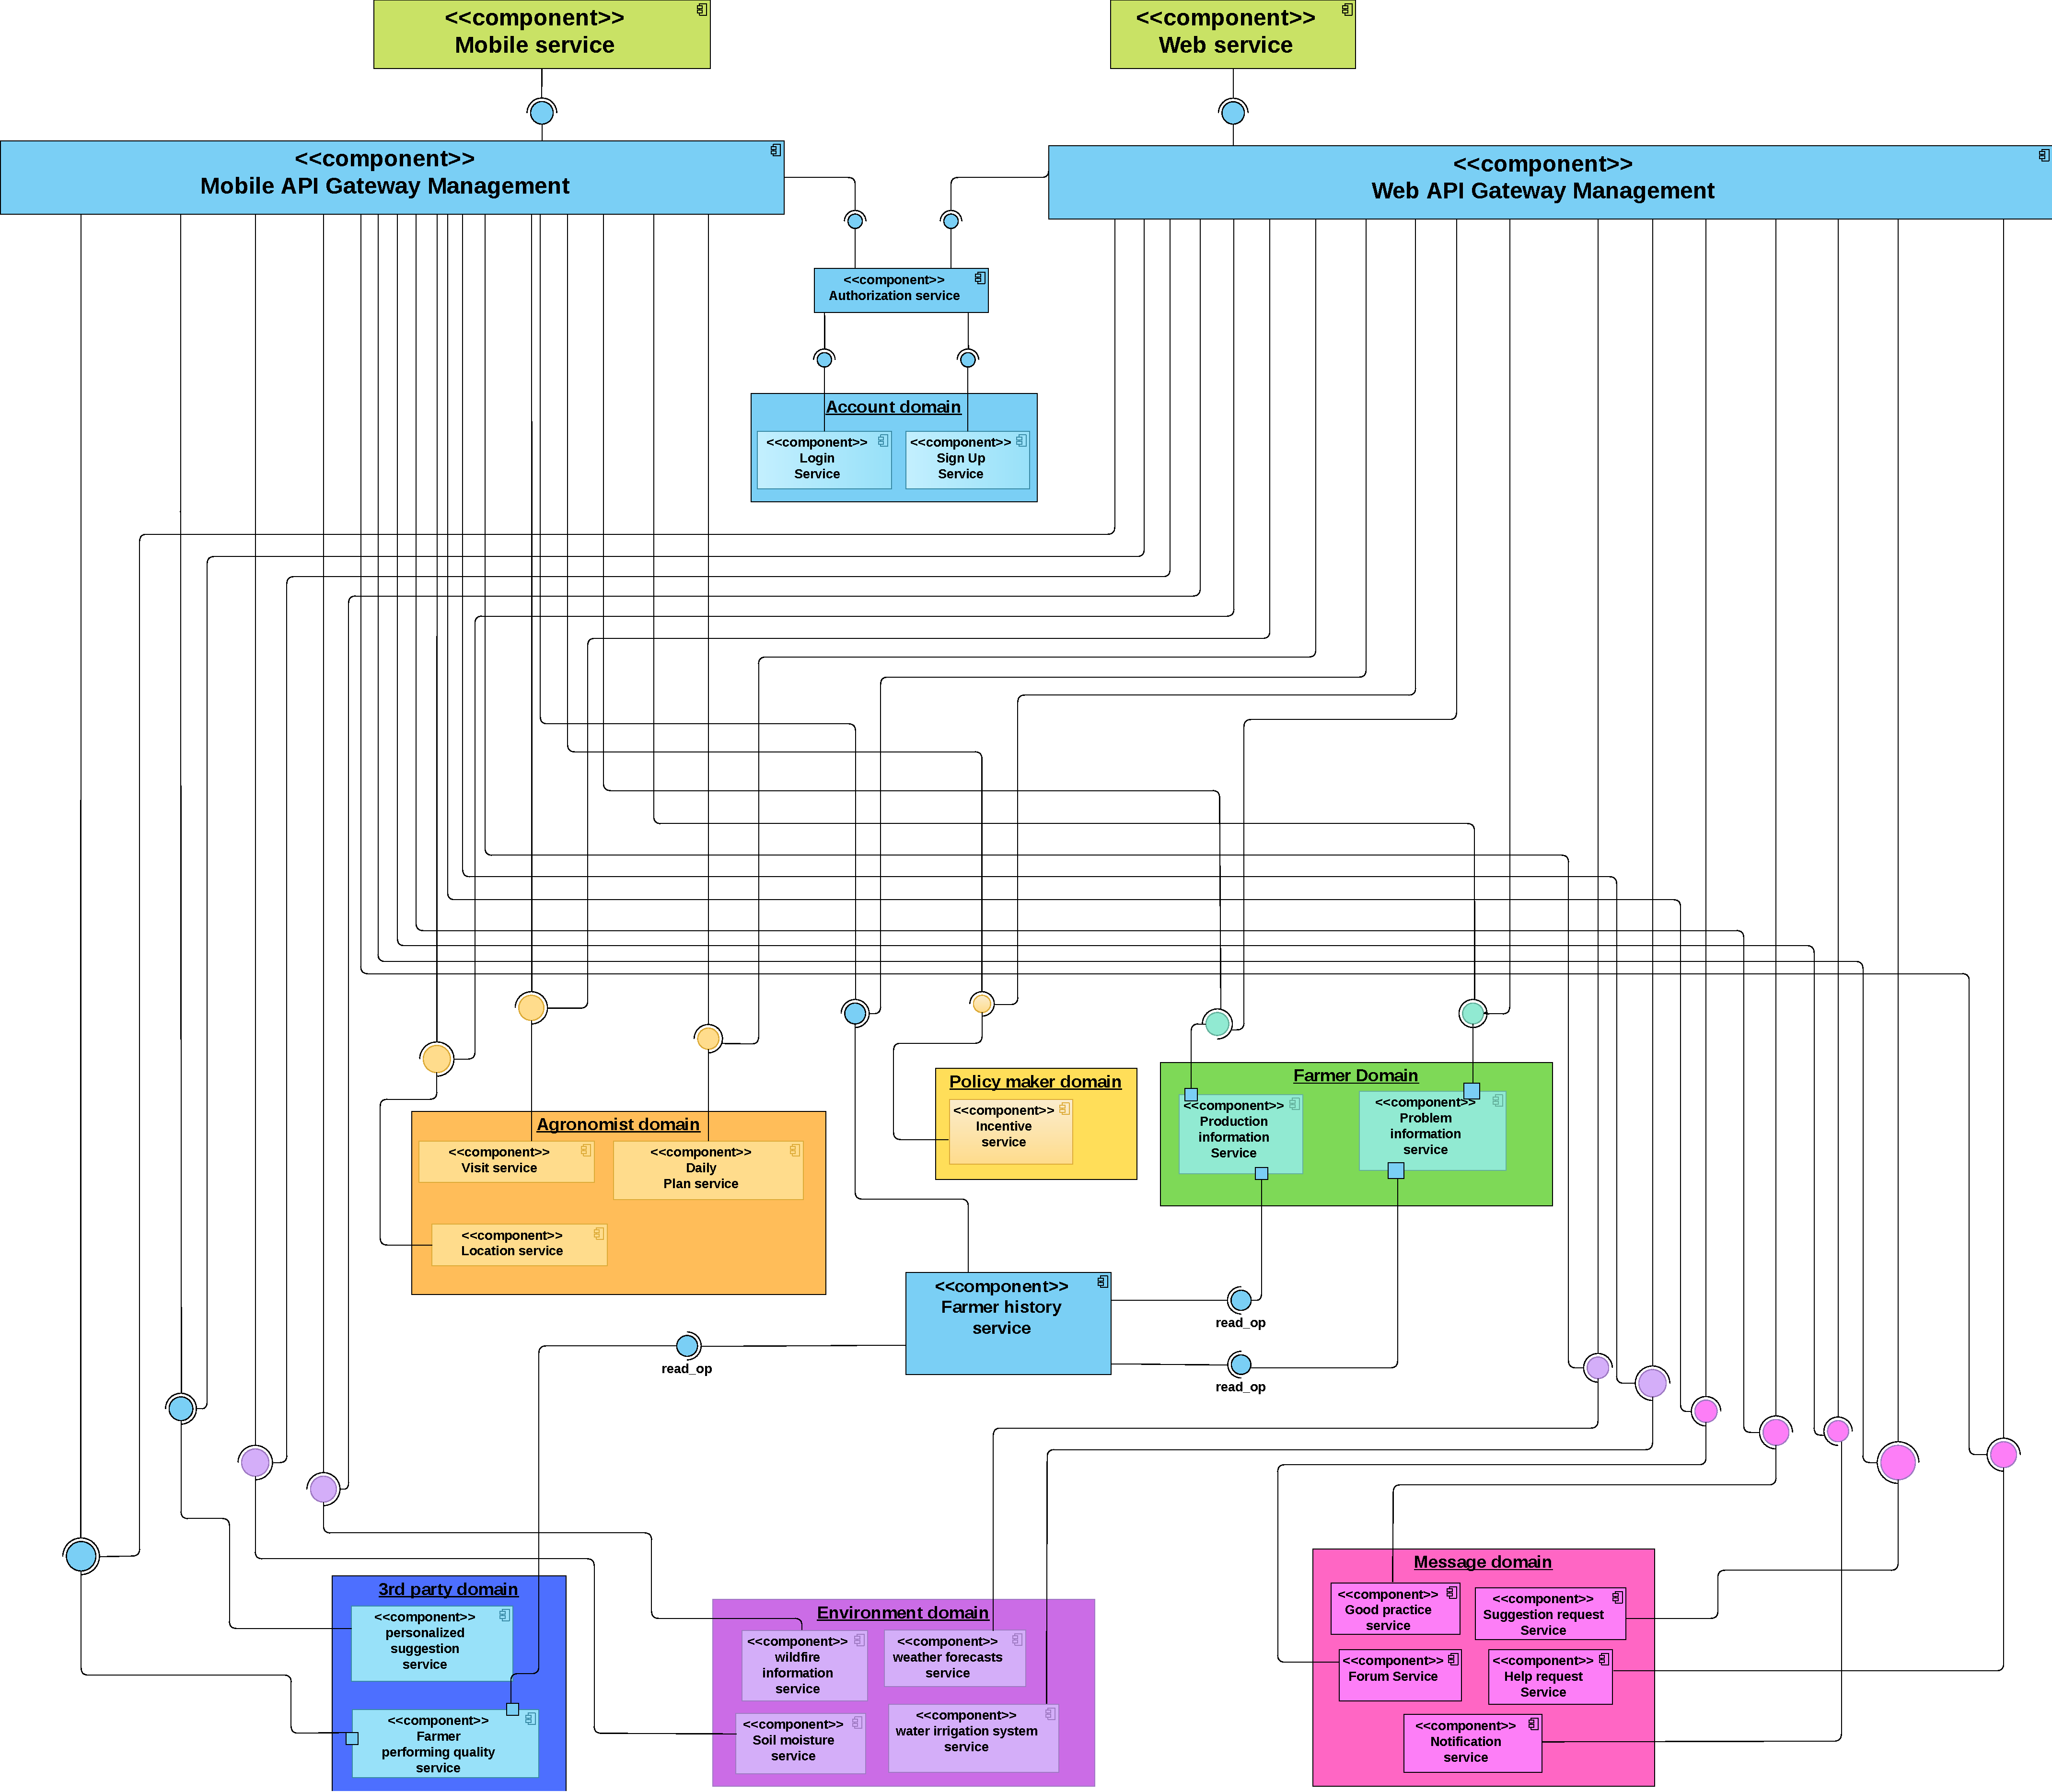
\includegraphics[width=0.99\paperwidth]{Images/Component Diagram2.pdf}}
    \caption{\label{fig:component_diagram}Component diagram}
\end{figure}

In figure \ref{fig:component_diagram} the platform is decomposed in 7 main domains:
\begin{itemize}
    \item The \textsc{\textcolor{cyan}{Account}} domain contains all the features in order to manage the user side. In fact, it includes the log in and sign up microservices. Moreover, the component provides different interfaces for different users, in order to provide additional distinct information.
    \item The \textsc{\textcolor{pink}{Message}} domain handles all different kind of message information exchanged between users, from simple suggestion and help requests to forum and good practice document requests. These microservices are completely used by farmers, and partially used by both agronomists and policy makers.
    \item The \textsc{\textcolor{purple}{Environment}} domain contains microservices that handle all the available environment information gathered by sensors along the state of Telangana. The four microservices contained in this domain manage the information of the water irrigation system, of the soil moisture, of the weather forecasts and the wildfire ones.
    \item The \textsc{\textcolor{blue}{3rd Party}} domain provides statistics mainly based on farmers information and the integration with the environment service information. This module is composed by two microservices responsible to provide reliable farmer's performance quality information and personalized suggestion.
    \item The \textsc{\textcolor{green}{Farmer}} domain contains farmer related CQRS-based microservices providing CRUD operations for production and problem information.
    \item The \textsc{\textcolor{orange}{Agronomist}} domain contains those microservices that fulfill agronomist requirements. In particular they provide utilities for managing the area they are responsible of, the daily plan and the visits confirmation.
    \item The \textsc{\textcolor{yellow}{Policy maker}} domain is composed by a single main microservice that is responsible to provide the incentive assignment functionalities.
    \item Finally, the Farmer history microservice provides READ only operations. This component uses event handlers that subscribe to events published by Farmer and 3rd party domains' services in order to keep its database updated.
\end{itemize}


% microservice integration is not anymore based on \textit{Enterprise Service Bus} (ESB) but they rely on \textit{smart endpoints and dumb pipes} style.

% source: https://medium.com/@nathankpeck/microservice-principles-smart-endpoints-and-dumb-pipes-5691d410700f

% 2.3
\subsection{Deployment view}
\label{sec:deployment_view}
% ############### 2.3) DEPLOYMENT VIEW ####################

In this section we describe the environment in which the system is executed from the perspective of the deployment diagram. Figure \ref{fig:deployment_diagram} shows the structure of the hardware components that execute the software, and presents the architecture in a more detailed way.


\begin{figure}[H]
    \makebox[\textwidth]{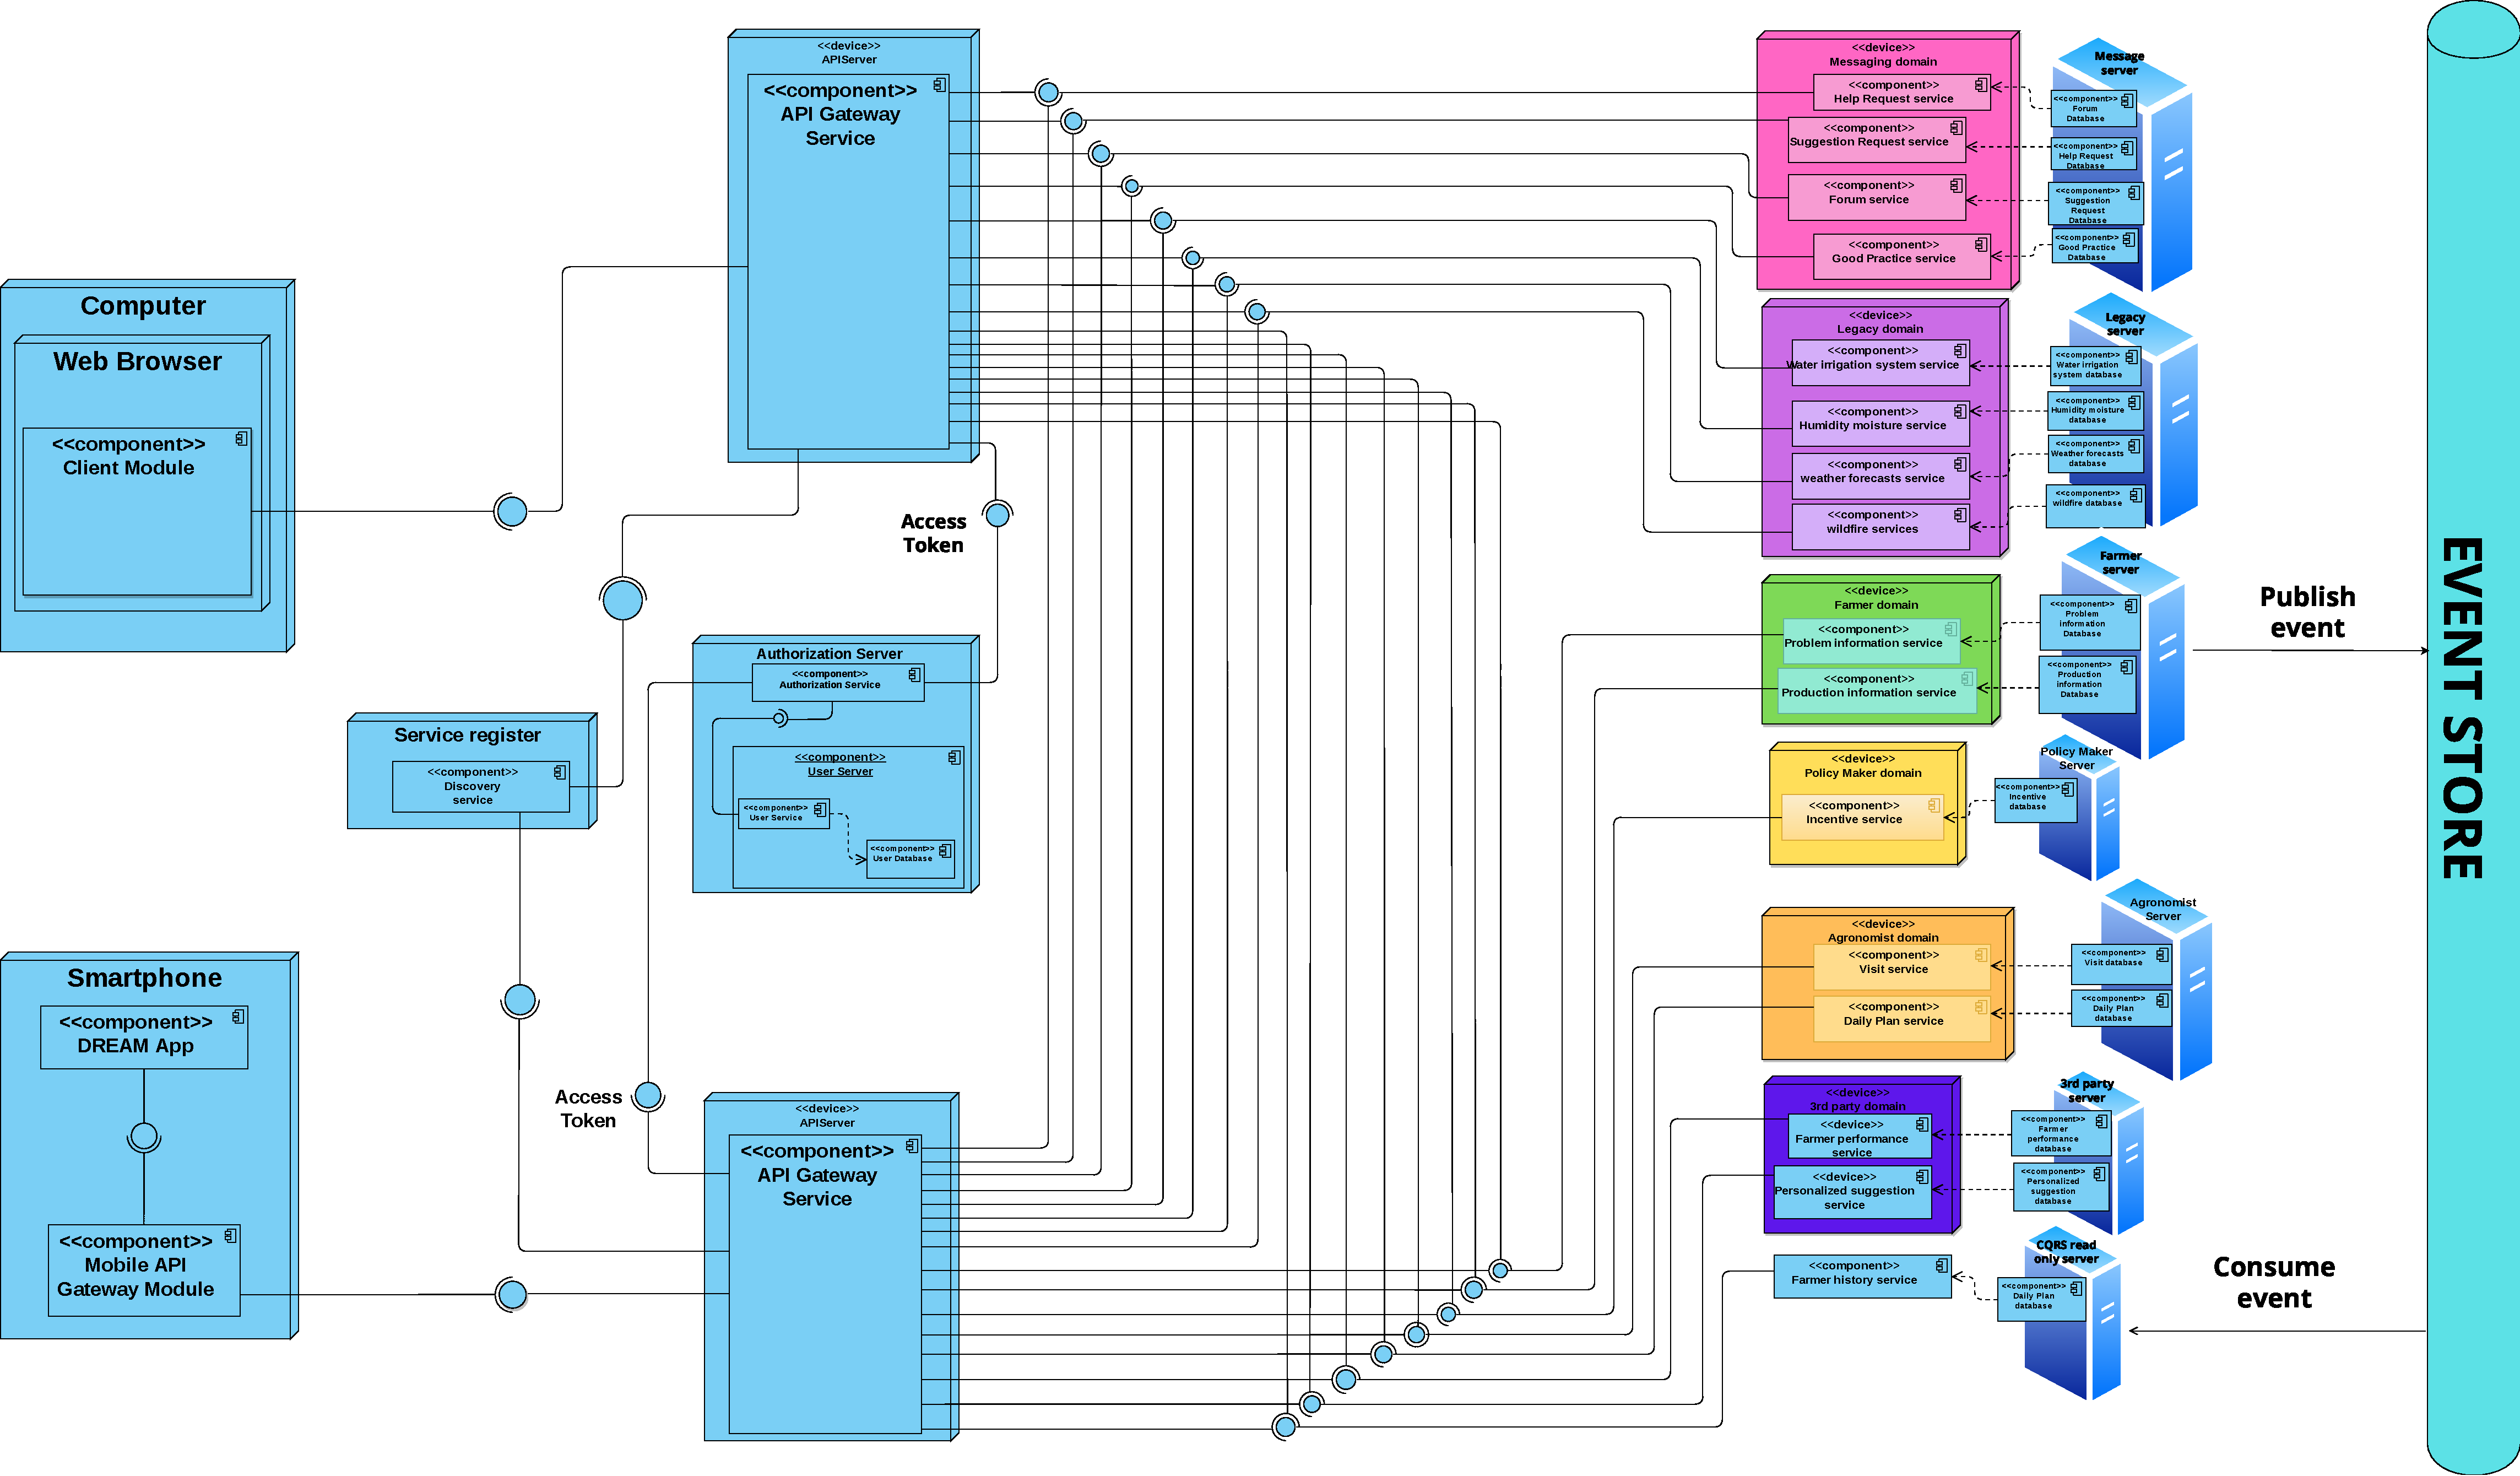
\includegraphics[width=\textheight, angle=90]{Images/deployment diagram.pdf}}
    \caption{\label{fig:deployment_diagram}Deployment diagram diagram}
\end{figure}

The above diagram highlights the four tiers of the architecture, and the relationship between components. In particular:
\begin{itemize}
    \item The \textsc{Presentation tier} is the front layer of the architecture and provides the final user interface (more details in section \ref{sect:user_interface_design}). As described in the RASD, the platform will be achievable through either an online web application or an installable mobile application. The web page's UI is supposed to provide both mobile and desktop visualization modes. This layer communicates with the application tier through API calls on HTTPS.
    \item The \textsc{routing tier} is composed by the API gateway pattern, which acts as the entry point of the application from the outer world. It is responsible mainly for request routing and protocol translation. It is similar to the Facade pattern from object-oriented design Like a facade, an API gateway encapsulates the application’s internal architecture and provides an API to its clients \cite{richardson2018microservices}. In addition to these functionalities, it is common practice to introduce in the API gateway pattern edge functionalities such as: authentication (Verifying the identity of the client making the request) and authorization (Verifying that the client is authorized to perform that particular operation) services, made possible through the introduction in the architecture of the authorization server component. Finally, in order to provide the service discovery pattern, a service registry component is required.
    \item The \textsc{business tier} contains the cloud of microservices that runs the core functionalities of the S2B. These ones are the same described in section \ref{sec:component_view} and communicate with the routing layer through RESTful APIs. Each microservice is responsible of a portion of the business logic and refer to its own database. Furthermore, microservices contained in the same domain (defined in the decomposition presented in section \ref{sec:component_view}) can be stored in the same server.
    \item Finally the \textit{data tier} contains the DBMS servers that store the data and provide SQL queries from the related microservices that communicate through an \textit{event store} for the implementation of the database management patterns (more details in section \ref{sec:styles_patterns}). This final tier could be implemented according to the \textbf{single service per container} or the \textbf{serverless} patterns.
\end{itemize}


\newpage
% 2.4
\subsection{Runtime view}
\label{sec:runtime_view}
% ############### 2.4) RUNTIME VIEW ####################

For letting diagram simpler, we supposed that all the example below are operations of success version (without considering any exceptions, every actor inserts the data correctly and satisfies their authorization requirements).
\newline
Additionally we also note that API gateway does a communication with authorization server to generate a token to let users execute only the ones they have permission to do. 


\begin{figure}[H]
	\centering
    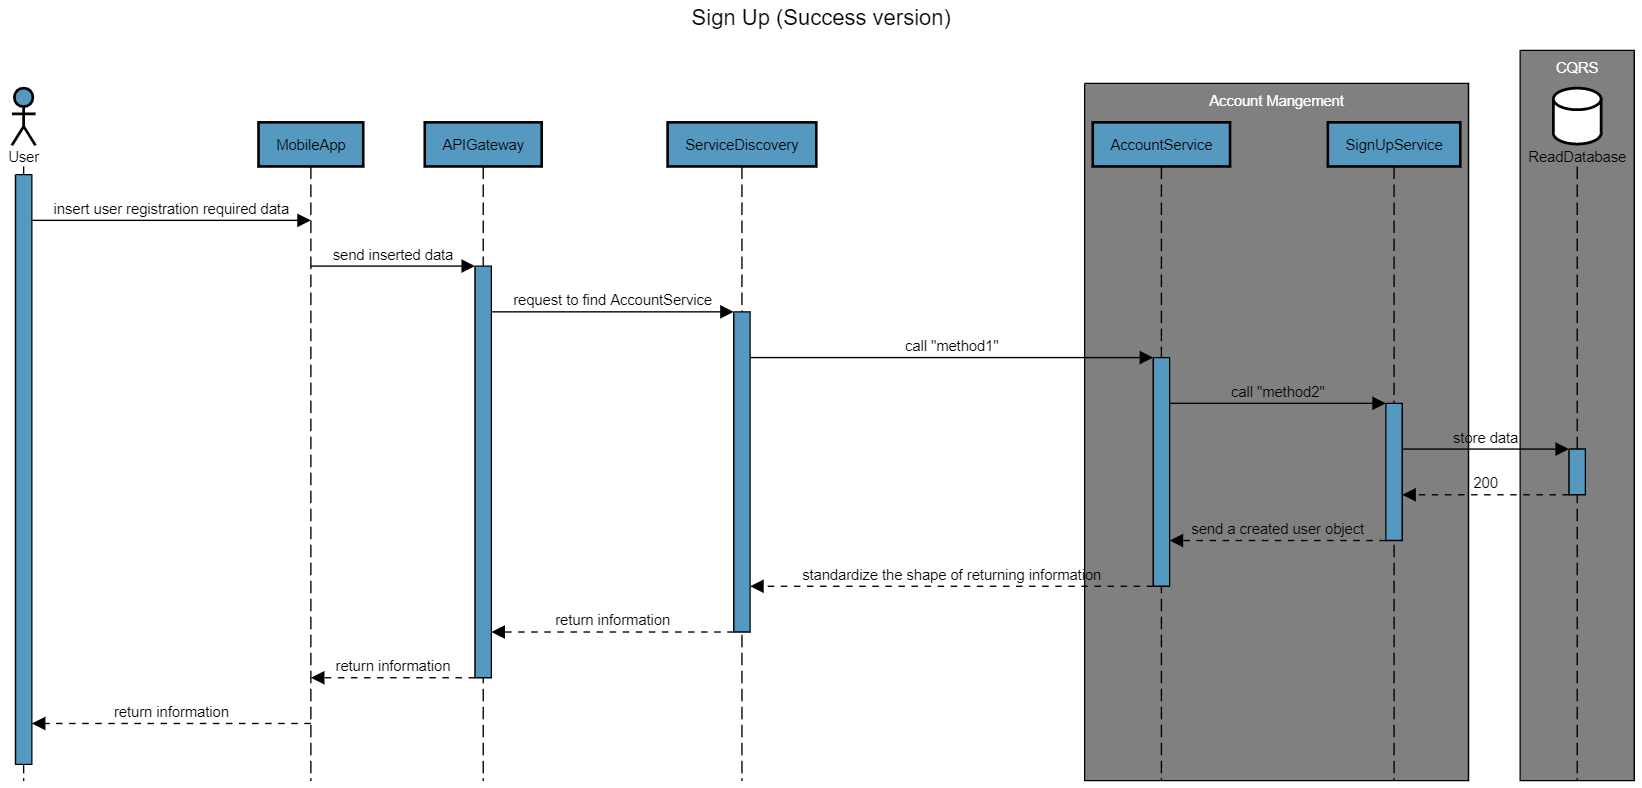
\includegraphics[width=\textwidth]{Images/sequence-diagram/sign-up.png}
	\caption{\label{fig:se_sign_up}Sign Up}
\end{figure}
Actor: All type of user
\newline
UI flow: {\ref{sec:user_mobile_interface} Sign Up, Login}

Firstly this diagram explains the flow of sign up for all type of user. 
Due to CQRS pattern, there are two different database according to their purpose (\ref{sec:component_view}). 
\newline
\textsc{\textcolor{blue}{flow overview}}

Mobile App sends a method ”postUser()” to Mobile Api Gateway, then service discovery does a job to find a routing path by URL of REST api.
Then SignUpService receives post request, after that for updating the database, since it is write operation, it sends command to Command handler to insert the data into Command DB. 

\newpage
\begin{figure}[H]
	\centering
    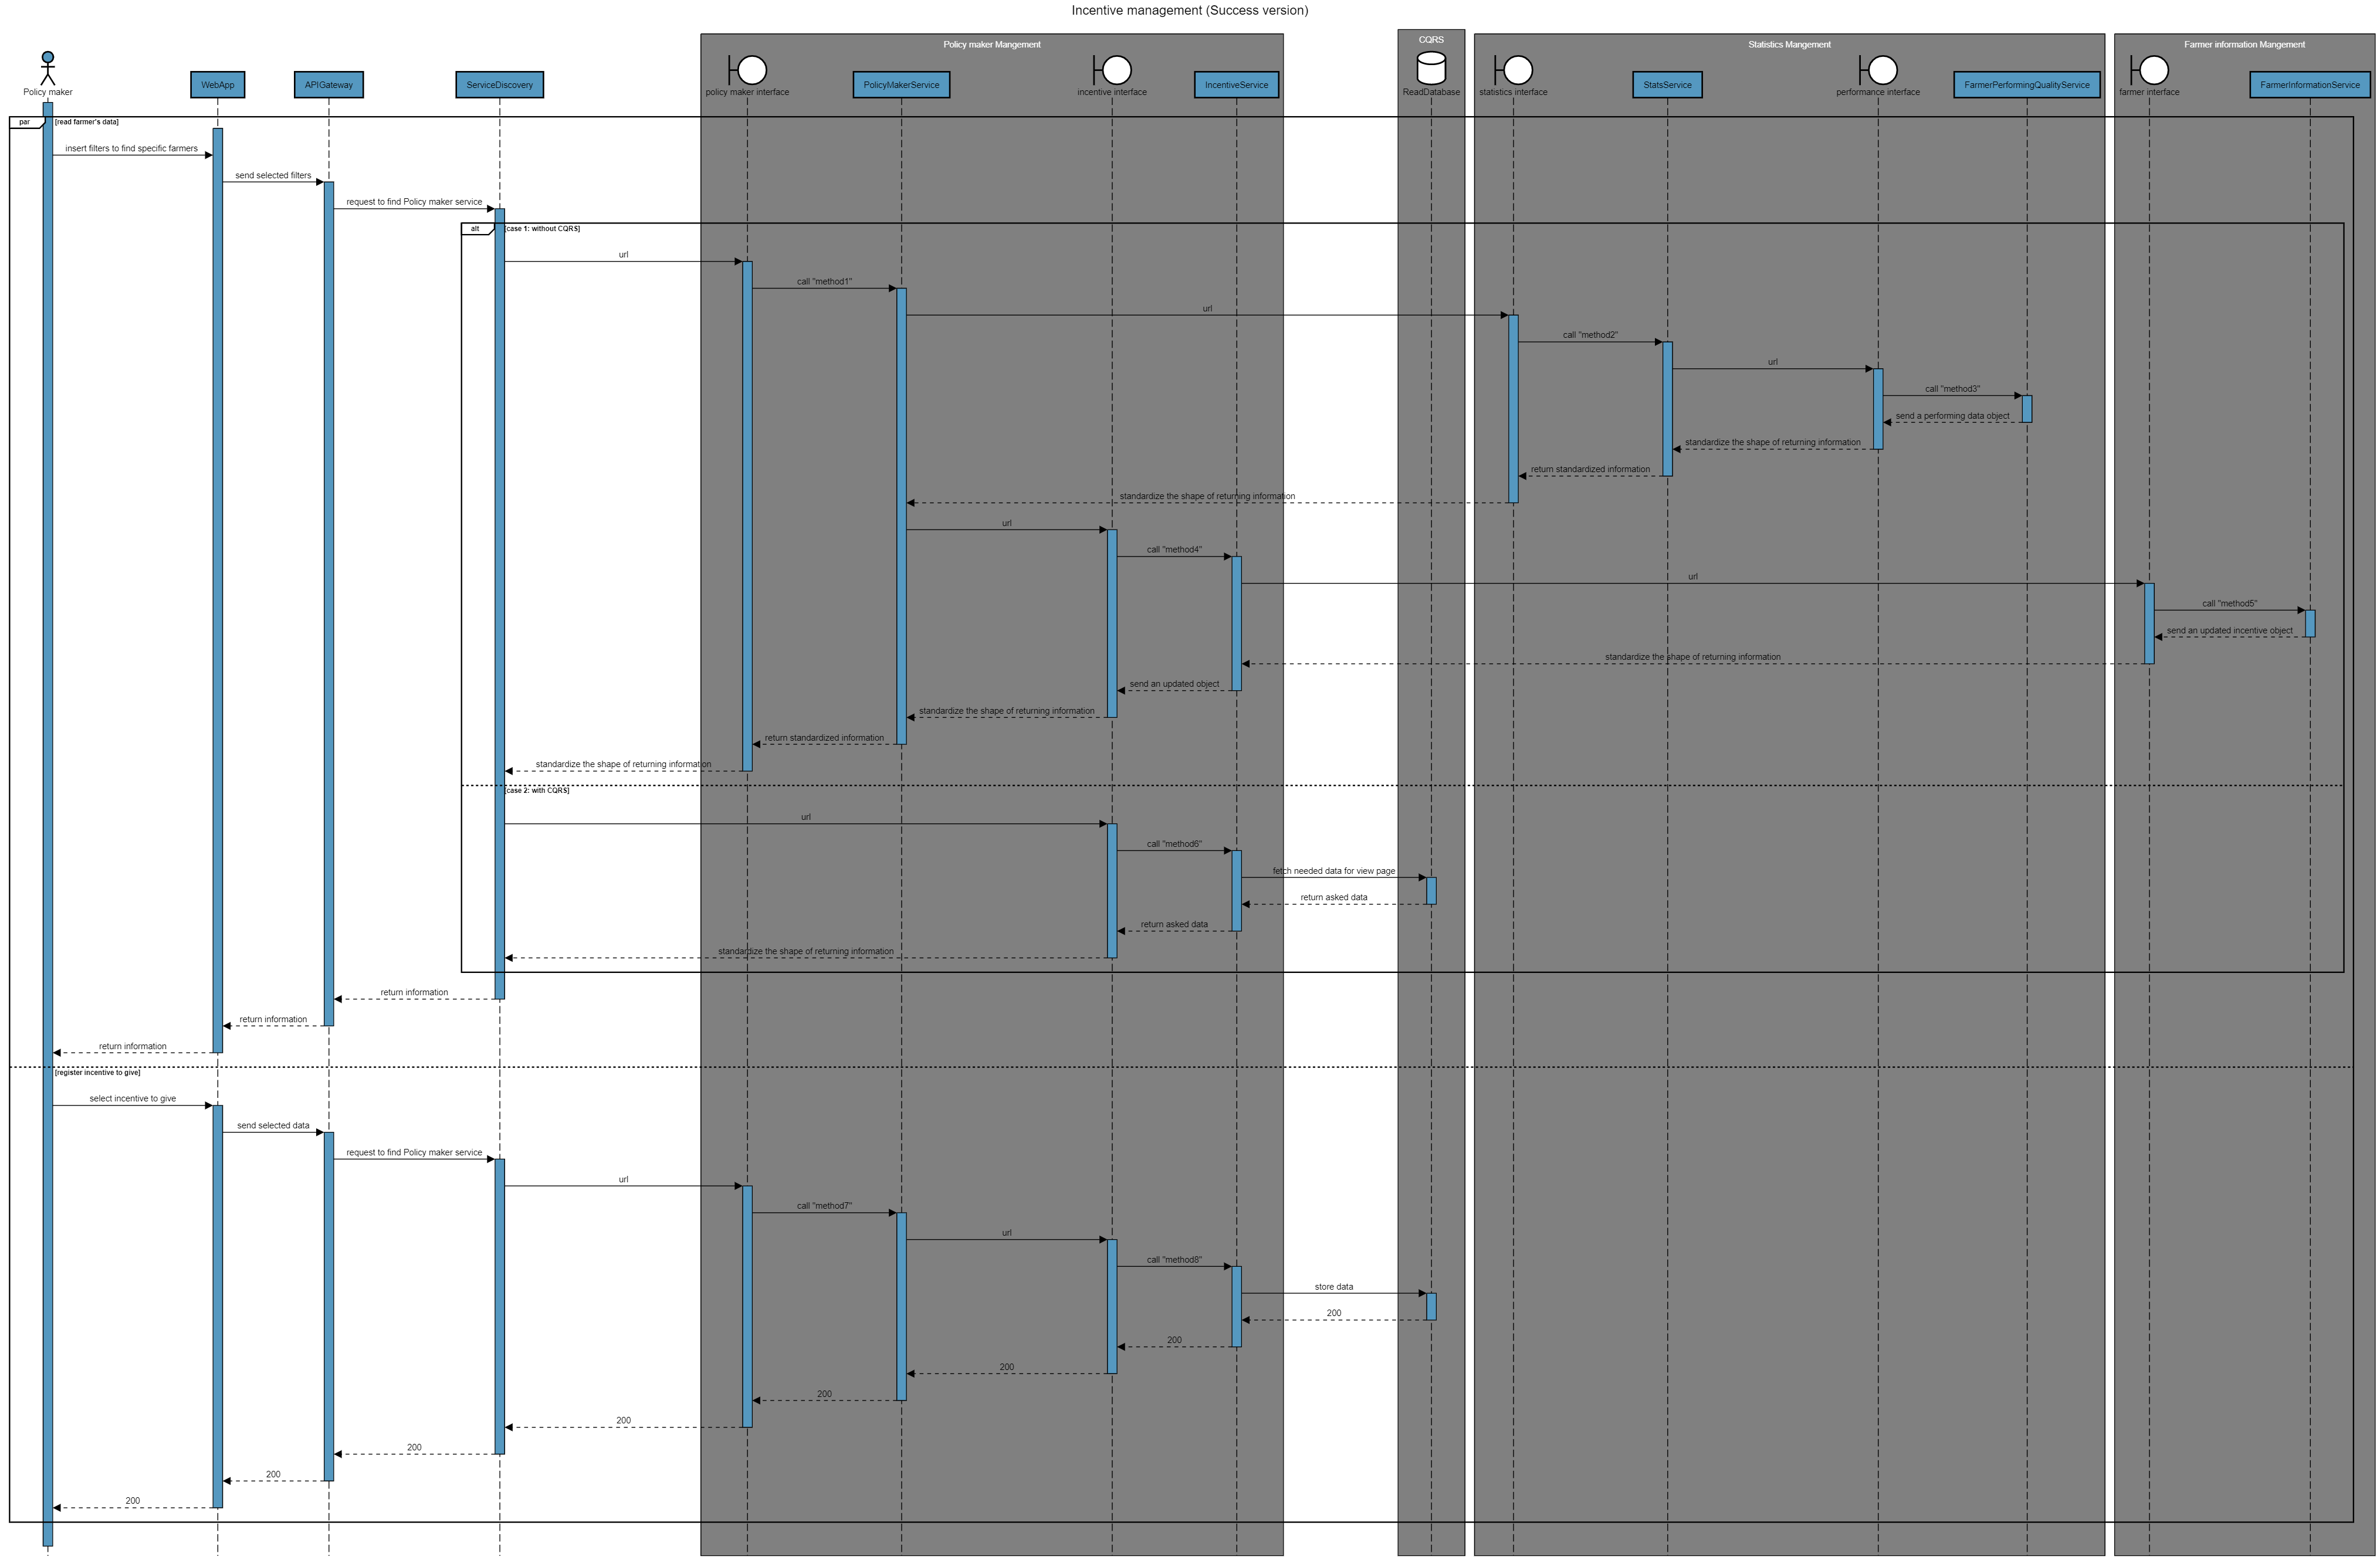
\includegraphics[width=\textwidth]{Images/sequence-diagram/incentive-management.png}
	\caption{\label{fig:se_incentive}Incentive management}
\end{figure}
Actor: Policy maker
\newline
UI flow: {\ref{sec:pm_web_interface} Farmer's performance data}

Secondly on this diagram, we would like to highlight about the reasoning of our design decision. We utilized CQRS pattern though, here it shows a comparison of each flow, one with CQRS pattern architecture, another without it.
By the fact we consider the analysis part taken cared by 3rd party systems, it also suits to have replica of database to fetch aggregated data when it is needed regardless of condition of their system.
\newline
\textsc{\textcolor{blue}{flow overview}}
\newline
Above part describes the flow of read operation. Search and show the data from database, it is required to access Query DB.
Then the below part explains the flow of write operation.
Incentive service needs to call Notification service to let the farmer who is selected to receive it.

\newpage
\begin{figure}[H]
	\centering
    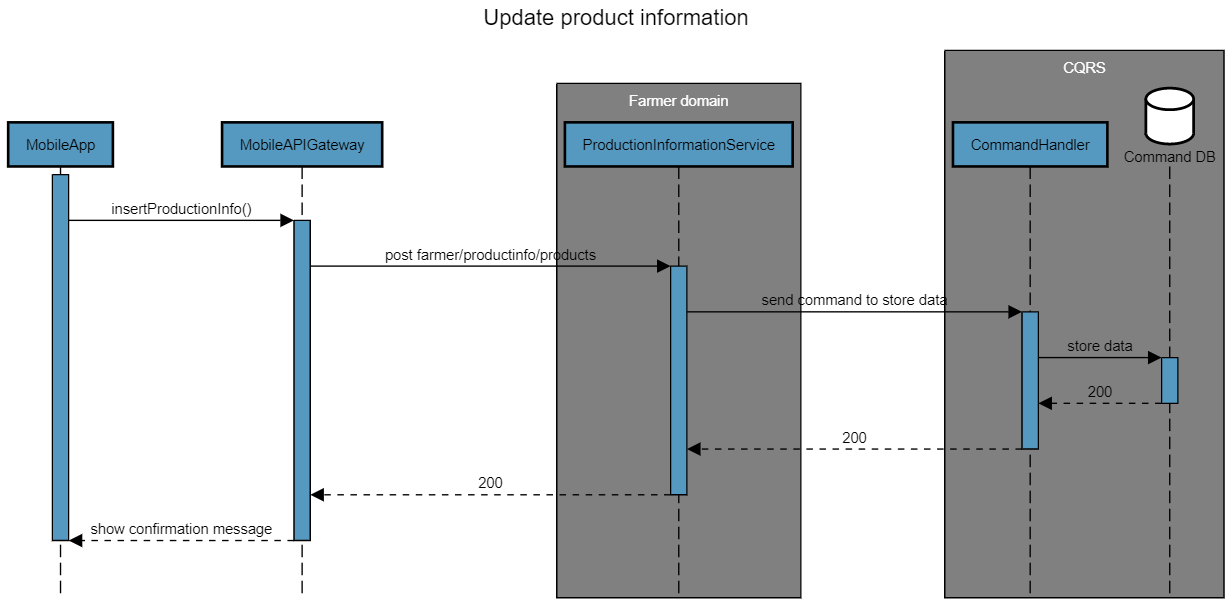
\includegraphics[width=\textwidth]{Images/sequence-diagram/product-info.png}
	\caption{\label{fig:se_product}Product information registration}
\end{figure}
Actor: Farmer
\newline
UI flow: {\ref{sec:farmer_mob_interface} Production data registration, Help/Suggestion request}

From this diagram, we consider API gateway component contains the operation to communicate with discovery service to find the suitable service location, besides that we also expect that each service has interfaces right before receiving a request as they are shown in two examples above (sign up, incentive management).
\newline
\textsc{\textcolor{blue}{flow overview}}
\newline
Farmer inserts needed information and send the production data to register it. API gateway contacts to authorization server to assure the permission, if it is verified, then discovery service finds ProductInformationService and execute the method. Since it is write operation, it sends data to Command handler to insert into Command DB.  

\newpage
\begin{figure}[H]
	\centering
    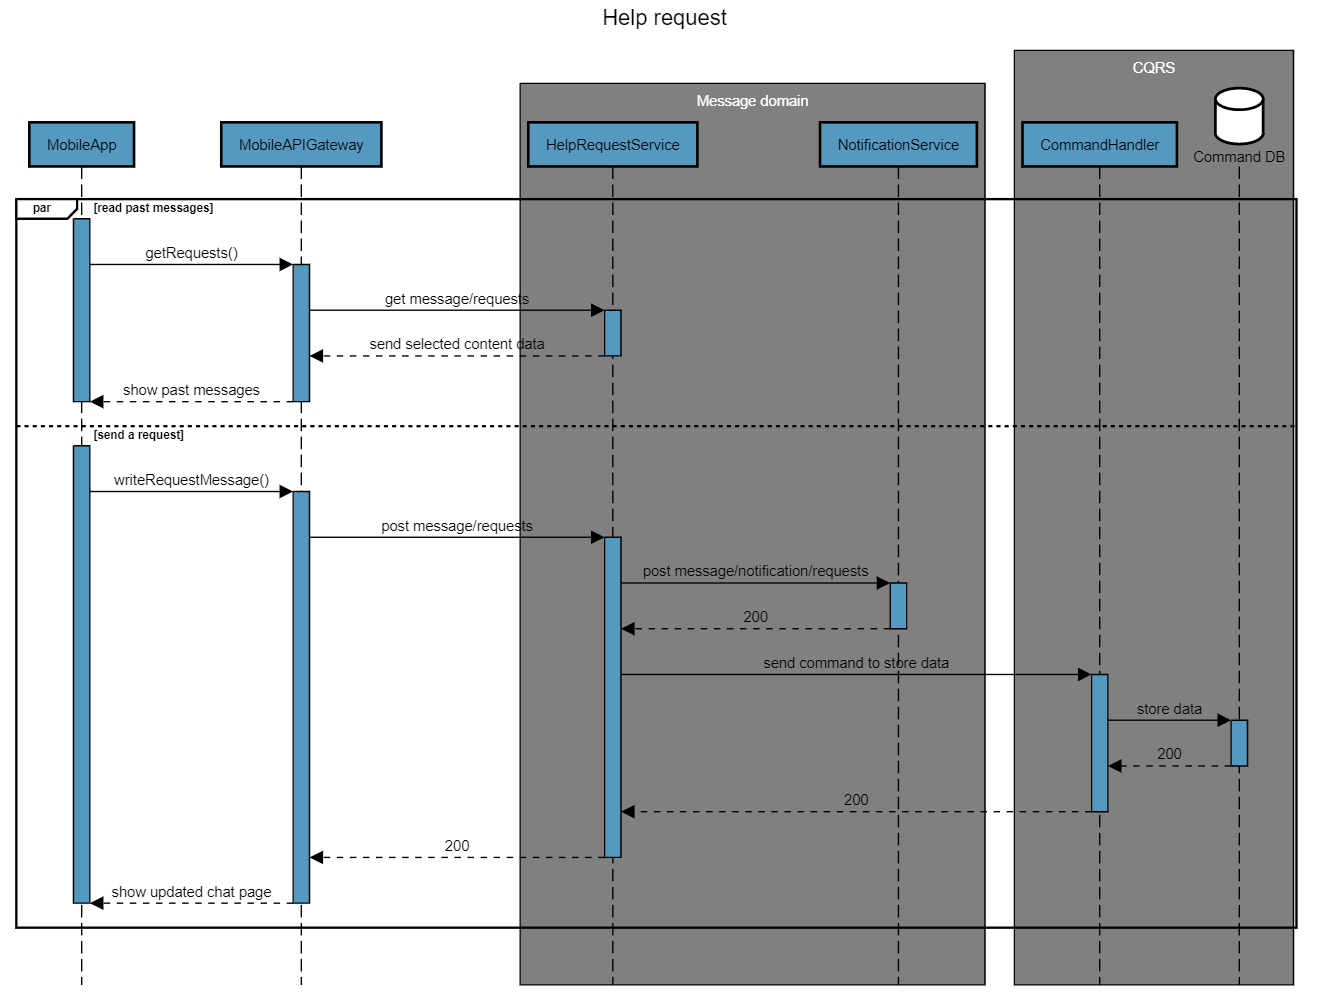
\includegraphics[width=\textwidth]{Images/sequence-diagram/help-request.png}
	\caption{\label{fig:se_help}Help request registration}
\end{figure}
Actor: Farmer
\newline
UI flow: {\ref{sec:farmer_mob_interface} Production data registration, Help/Suggestion request}

This diagram explains the flow of asking help request.
As a previous step, it requires farmer to select whom they would like to ask though, we assumed this operation has been done in advance and the diagram above describes the phase afterwards.
\newline
\textsc{\textcolor{blue}{flow overview}}
\newline
First half shows the flow of read operation to visualise the past messages, on the other hand the below part represents the write operation to send the message. 
For read operation it does not access to Query DB since the data is not aggregated data, it simply access the database inside of own service.

\newpage
\begin{figure}[H]
	\centering
    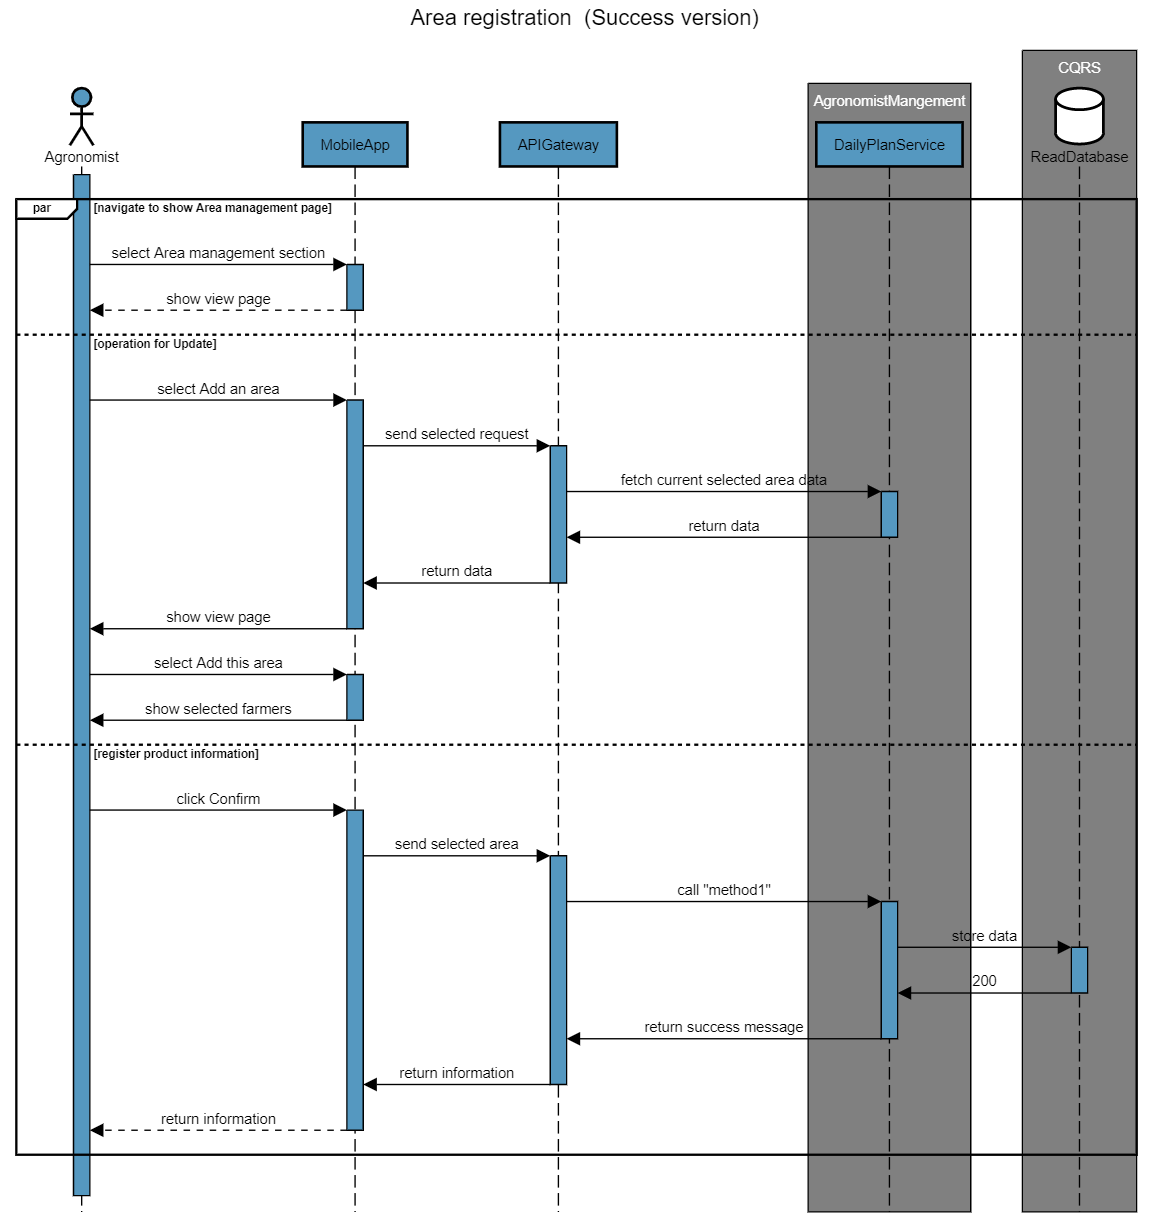
\includegraphics[width=\textwidth]{Images/sequence-diagram/area-registration.png}
	\caption{\label{fig:se_area}Area registration}
\end{figure}
Actor: Agronomist
\newline
UI flow: {\ref{sec:agronomist_mob_interface} Area management}

This diagram shows the flow of registering new area to supervise. As like other examples, this diagram contains read and write operation individually.

\textsc{\textcolor{blue}{flow overview}}
\newline
Firstly by calling getAreas(), it will fetch current area information about the place(name of farmers, agronomist). After agronomist observe area information and if they are interested in they could register a new area to supervise it. Write operation require to update Command DB to let new registered data be reachable by other services.

\newpage
\begin{figure}[H]
	\centering
    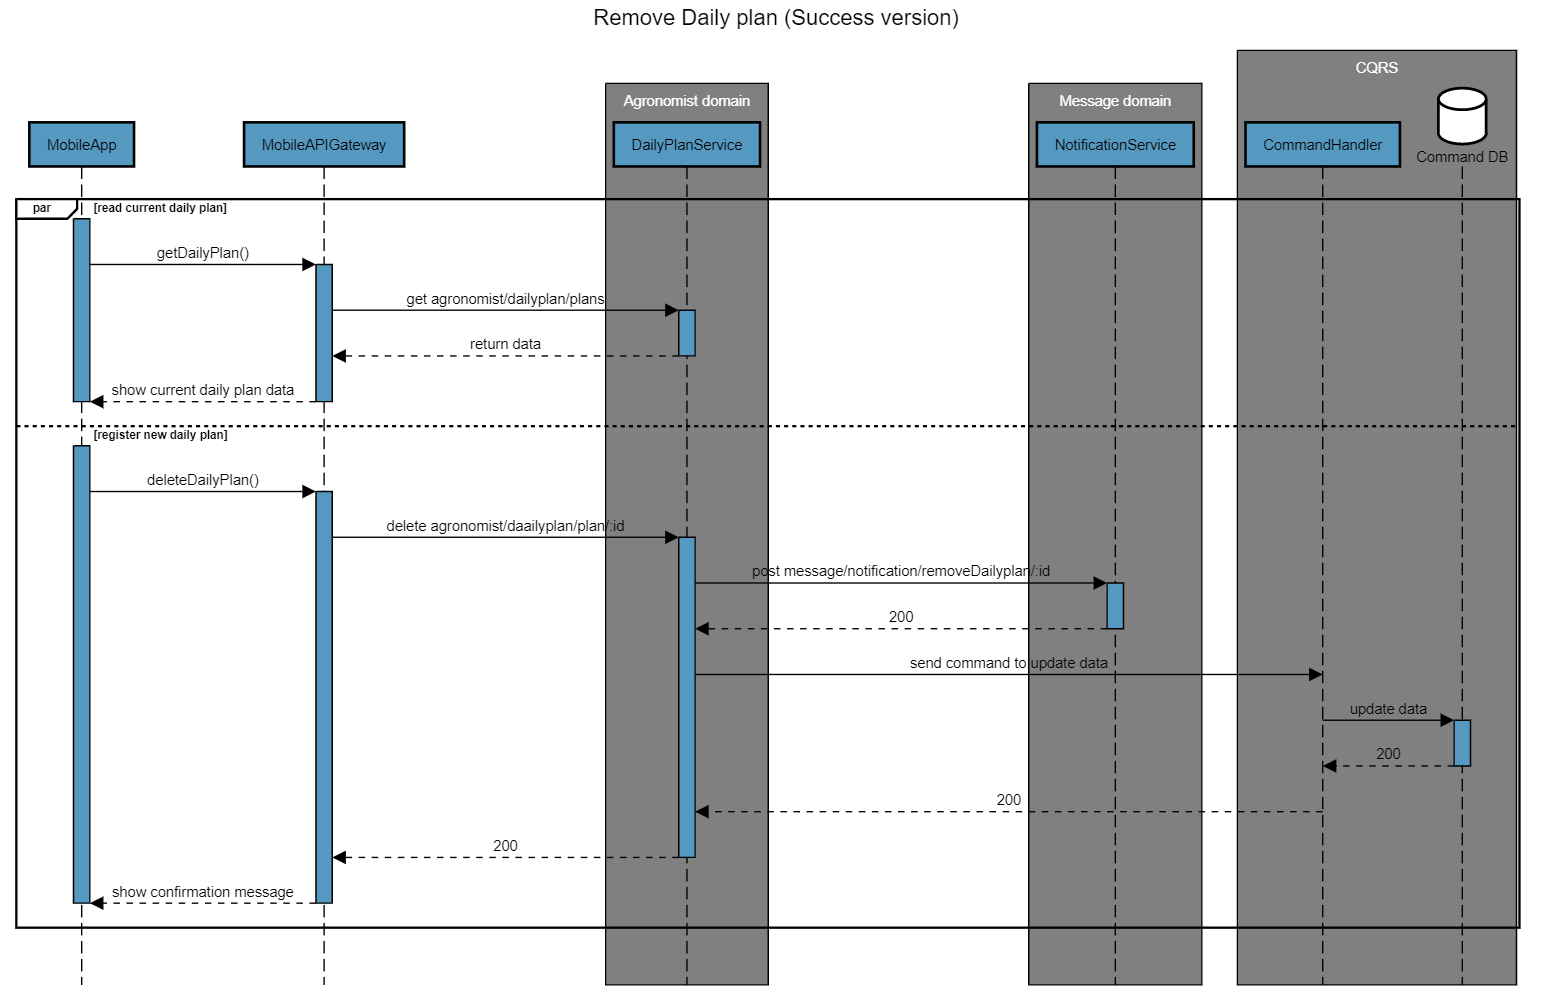
\includegraphics[width=\textwidth]{Images/sequence-diagram/daily-plan.png}
	\caption{\label{fig:se_daily}Remove Daily plan}
\end{figure}
Actor: Agronomist
\newline
UI flow: {\ref{sec:agronomist_mob_interface} Daily plan management}

As a last example, this diagram shows the flow of updating daily plan of agronomist.
Unlike other insertion examples, here it deletes the record from database, so it requires DELETE method.
\newline
\textsc{\textcolor{blue}{flow overview}}
\newline
On the upper part it let agronomist know the daily plan they have. Instead, the bottom explains the flow of deletion operation. Specifying id in url, Command Handler searches the record owns that id and it deletes the one matches. 

% 2.5
\subsection{Component interfaces}
\label{sec:component_interfaces}
% ############### 2.5) COMPONENT INTERFACES ####################

interfaces diagram, interfaces description

% 2.6
\subsection{Architectural styles and patterns}
\label{sec:styles_patterns}
% ############### 2.6) ARCHITECTURAL STYLES AND PATTERNS ####################

\subsubsection{Microservice Architecture}
The S2B will be implemented using Microservice architecture, an architectural style that breaks the business logic into small and independent modules. 
\newline
\newline
Adopting a microservice-based approach grants many benefits:
\begin{itemize}
    \item modularity: this makes the software easier to understand, develop, test, and become more resilient to architecture erosion; this aspect is very important for complex systems such as DREAM.
    \item scalability: since microservices are implemented and deployed independently of each other (i.e. they run within independent processes), they can be monitored and scaled independently; scalability is a crucial aspect for DREAM, considering the wide user base and the possibility of future expansions.
    \item distributed development: development can be parallelized, enabling small autonomous teams to develop, deploy and scale their respective services independently; it also allows the architecture of an individual service to emerge through continuous refactoring; in general, microservice-based architectures facilitate continuous integration, continuous delivery and deployment.
    \item digital public good fitting: since DREAM tries to follow the Digital Public Good principles (being the product of a United Nations initiative), a microservice architecture enables the system to be well-structured and to adopt open APIs with great flexibility.
\end{itemize}

\subsubsection{RESTful Architecture}
The S2B will adopt the REST (Representational state transfer) architecture, which is based on the concept of stateless sessions and connections. Since each application is designed as an independent service, REST is a valuable architectural style for microservices, thanks to its simplicity, flexibility, and scalability. 

One of the strongest advantages of REST for microservices is that services can communicate without requiring internal knowledge of one another. Furthermore, in RESTful microservices, APIs are standardized according to the OpenAPI Specification, which provides a documented contract for how services are expected to communicate across ongoing development.

\subsubsection{API Gateway}
The API gateway pattern is very often used in Microservice architecture to handle the complexity of a distributed and fragmented system. The API gateway represents the single entry point for all clients. It handles requests in one of two ways: some requests are simply proxied/routed to the appropriate service, while other requests are fanned out to multiple services. 

Moreover, rather than provide a one-size-fits-all style API, the API gateway can expose a different API for each client (i.e. Web app API gateway, Mobile API gateway, Public API gateway). This pattern allows to simplify the client’s logic by hiding the microservice structure internally and by handling multiple service calls server-side.

\subsubsection{Event Sourcing}
Given the fragmented nature of microservices, a service must atomically update the database and send messages in order to avoid data inconsistencies and bugs.  Event sourcing persists the state of a business entity as a sequence of state-changing events. Whenever the state of a business entity changes, a new event is appended to the list of events. The application can reconstruct an entity’s current state by replaying the events.

Applications persist events in an event store, which is a database of events. The store has an API for adding and retrieving an entity’s events. The event store also behaves like a message broker. It provides an API that enables services to subscribe to events. When a service saves an event in the event store, it is delivered to all interested subscribers.

This particular pattern is required from other patterns used in the overall database management process.

\subsubsection{Domain Event}
Since a service often needs to publish events when it updates its data, the Domain Event pattern is used to organize the business logic of a service as a collection of DDD (Domain-Driven Design) aggregates that emit domain events when they are created or updated. The service publishes these domain events so that they can be consumed by other services. 

This pattern is required from other patterns used in the overall database management process, such as CQRS and Saga.

\subsubsection{Database per Service}
The Database per Service pattern is used to keep each microservice’s persistent data private to that service and accessible only via its API. In this way, the service’s database is effectively part of the implementation of that service and it cannot be accessed directly by other services.

Depending on the resources available for the real deployment of the system, there are different ways to keep a service’s persistent data private:
\newline
- Private-tables-per-service: each service owns a set of tables that must only be accessed by that service
\newline
- Schema-per-service: each service has a database schema that’s private to that service
\newline
- Database-server-per-service: each service has its own database server

It is a good idea to create barriers that enforce this modularity. Without some kind of barrier to enforce encapsulation, developers may be tempted to bypass a service’s API and access its data directly.

In this document we assumed an hybrid approach, as shown in section 2.3: different “domains” have different machines, but inside each machine a logical separation is used.

\subsubsection{Saga}
This pattern implements each business transaction that spans multiple services as a saga. A saga is a sequence of local transactions. Each local transaction updates the database and publishes a message or event to trigger the next local transaction in the saga. 

If a local transaction fails because it violates a business rule, then the saga executes a series of compensating transactions that undo the changes that were made by the preceding local transactions.

To coordinate these sagas, a choreography approach may be chosen: each local transaction publishes domain events that trigger local transactions in other services.

The Saga pattern enables the application to maintain data consistency across multiple services without using distributed transactions.

\subsubsection{CQRS (Command Query Responsibility Segregation)}
Given the fragmented nature of microservices, it is no longer straightforward to implement queries that join data from multiple services. 

The Command Query Responsibility Segregation (CQRS) pattern defines a view database, which is a read-only replica that is designed to support that query. The application keeps the replica up to data by subscribing to Domain events published by the service that own the data. 

This pattern works together with other patterns in the overall database management process.

\subsubsection{Access Token}
The Access Token pattern is used for security reasons, in order to communicate the identity of the requestor to the services that handle the request. The API Gateway authenticates the request through an Authorization server and passes an access token (e.g. JSON Web Token) that securely identifies the requestor in each request to the services. 

A service can include the access token in requests it makes to other services. In this way, the identity of the requestor is securely passed around the system and the services can verify that the requestor is authorized to perform a specific operation, especially when accessing data resources.

\subsubsection{Circuit Breaker}
The Circuit Breaker is used to efficiently handle synchronous calls to microservices in order to prevent a network or service failure from cascading to other services.
A service client invokes a remote service via a proxy. When the number of consecutive failures crosses a threshold, the circuit breaker trips, and for the duration of a timeout period all attempts to invoke the remote service will fail immediately. After the timeout expires the circuit breaker allows a limited number of test requests to pass through. If those requests succeed the circuit breaker resumes normal operation. Otherwise, if there is a failure the timeout period begins again.

This is due to the fact that, when one service synchronously invokes another, there is always the possibility that the other service is unavailable or is exhibiting such high latency it is essentially unusable, causing the caller to waste resources in the meanwhile.

\subsubsection{Server-side Discovery}
The Server-side Discovery pattern is used to manage the virtualized or containerized environment in which the microservice-based application runs, where the number of instances of a service and their locations changes dynamically.

With this pattern, when making a request to a service, the caller makes a request via a router (a.k.a load balancer) that runs at a well known location. The router queries a service registry, which might be built into the router, and forwards the request to an available service instance.

This pattern allows to keep the client code simpler, since it does not have to deal with discovery. In addition, the possibility of using virtualization inside the system’s modules increases the availability and the scalability of the software since it is possible to dynamically generate new service instances when needed.

\subsubsection{Monolithic front-end}
For the first implementation and deployment of the system, we decided to adopt a monolithic front-end that handles the calls to the system and puts together all the information gathered by querying the platform, thanks to its simplicity and easy deployment. A future implementation of micro front-ends is suggested in order to guarantee scalability also on the client side, increasing however the complexity of the software, but assuring easier updates for long-term operations. For this particular transition, the user experience could be retrieved through some sort of feedback mechanism in order to develop the most suitable application possible.


% 2.7
\subsection{Other design decisions}
\label{sec:other_decisionS}
% ############### 2.7) OTHER DESIGN DECISIONS ####################

\subsubsection{Scale-out}
This method consists of cloning the nodes in which we expect to have a bottleneck, in order to increase the overall availability and scalability of the system. In particular, elements such as the API gateway, the Authorization Server and the Discovery Service should necessarily  be replicated since they represent a single point of failure. 

Also the microservices can be replicated: the managing process of redirecting the incoming requests to the node with the lowest workload could be done in the load balancer already implemented in the Discovery Service (see 2.6.11 for more details).

\subsubsection{Thin and thick client}
The web application will be the thin client. This means that it will have only presentation duties, with no business logic inside. In this way, the machines that run the web application are not required to have high computational power. However, a stable internet connection is required to guarantee the proper usage of the application.

The mobile application, instead, will be the thick client. In fact, it is reasonable to save useful information on the local memory of the device (for example chats) in order to avoid continuous requests to the platform (less computational load) and to guarantee also some functionalities when the Internet connection is not available.




%------------------------------------------------------------------------------------------------------------------------------------------------
\clearpage
{\color{Blue}{\section{\label{sect:user_interface_design}User interface design}}}

% ############ 3.1) USER GUI ########################
\subsection{User mobile interface}
\label{sec:user_mobile_interface}

% ############ 3.1) USER GUI ########################

front-end flow diagram

% ############ 3.2) POLICY MAKER GUI ########################
\subsubsection{Policy maker web interface}
\label{sec:pm_web_interface}

% ############ 3.2) POLICY MAKER GUI ########################

\begin{figure}[H]
	\centering
    \includegraphics[width=\textwidth]{Images/UI/ui-2.pdf}
	\caption{\label{fig:bpmn_sign_up}Farmer's performance data}
\end{figure}

\begin{figure}[H]
	\centering
    \includegraphics[width=\textwidth]{Images/UI/ui-3.pdf}
	\caption{\label{fig:bpmn_sign_up}Effectiveness of initiatives}
\end{figure}

% ############ 3.3) FARMER GUI ########################
\subsubsection{Farmer mobile interface}
\label{sec:farmer_mob_interface}

% ############ 3.3) FARMER GUI ########################

\begin{figure}[H]
	\centering
    \includegraphics[width=\textwidth]{Images/UI/ui-4.pdf}
	\caption{\label{fig:ui_production}Production data registration, Help/Suggestion request}
\end{figure}
\newpage
\begin{figure}[H]
	\centering
    \includegraphics[width=\textwidth]{Images/UI/ui-5.pdf}
	\caption{\label{fig:ui_forum}Forum, Problem information}
\end{figure}

\begin{figure}[H]
	\centering
    \includegraphics[width=\textwidth]{Images/UI/ui-6.pdf}
	\caption{\label{fig:ui_practice}Good practice, relevant data}
\end{figure}

% ############ 3.4) AGRONOMIST GUI ########################
\subsubsection{Agronomist mobile interface}
\label{sec:agronomist_mob_interface}

% ############ 3.4) AGRONOMIST GUI ########################
front-end flow diagram \ldots



%------------------------------------------------------------------------------------------------------------------------------------------------
\clearpage
{\color{Blue}{\section{\label{sect:req_traceability}Requirements traceability}}}

(possible) requirements summary, requirements to component mapping

In addition, also the software system attributes (described in the RASD) are guaranteed by the architectural design choices made and explained in this document. 

In particular:
\begin{itemize}
    \item \textbf{Usability}: it is achieved through a simple and intuitive interface, as shown in section 3. The possible choices are clearly presented to the user, both in the mobile app and in the web application. With this simple type of interface, the application could be used by all types of users, for example also by elders and by people that are not very experienced with electronic devices.
    
    \item \textbf{Reliability and Availability}: they are accomplished through replication and the subdivision in microservices. Thanks to modularity and low coupling, possible problems are limited to a single microservice, without affecting others. Moreover, the replication of nodes allows the system to be even more fault tolerant, especially in critical elements such as the API gateway, the Authorization server, the Discovery Service and the shared read-only database. 

    \item \textbf{Security}: it is guaranteed through the Authorization Server and the Access Token pattern. Since the API gateway represents a single point of entrance, the identity of a user can be checked before forwarding his request to the microservices. Moreover, since the access token is passed around the system together with the request, a Role Based Access Protocol (RBAC) could be adopted because the information about the role of a user can be put inside the token. In addition, communication running on HTTP is encrypted thanks to protocols such as HTTPS and SSL.

    \item \textbf{Portability}: it is achieved through the implementation of a web application and the existence of an API gateway. The lightweight web application allows the system to be accessed from any device provided with an internet browser. The API gateway, instead, allows the development of a mobile app for different operating systems (mainly Android and iOS) thanks to the fact that it offers a dedicated interface for each client type, guaranteeing compatibility and providing additional elasticity to the developers.

    \item \textbf{Maintainability and Scalability}: they are accomplished through the Microservice architecture itself. A microservice-based approach grants high modularity and low coupling, with independent components that are easier to maintain, test and fix. Microservices also grant high scalability because new modules can constantly be added to the system for future upgrades, introducing new functionalities, without affecting the behaviour of the other components of the application.
\end{itemize}

%------------------------------------------------------------------------------------------------------------------------------------------------
\clearpage
{\color{Blue}{\section{\label{sect:impl_int_test}Implementation, integration and testing plan}}}

% ############ 5.1) IMPLEMENTATION PLAN ########################
\subsection{Implementation plan}
\label{sec:implementation_plan}

% ############ 5.1) IMPLEMENTATION PLAN ########################

In this section we present all the preliminary considerations needed to implement and test the S2B from the beginning of its life.
\newline
\newline
The S2B will be divided as follows:
\begin{itemize}
    \item Client (Web App and Mobile App)
    \item API gateway (with Discovery Service)
    \item Authorization Server
    \item Microservices
    \item Event BUS
    \item External services
\end{itemize}
 
A bottom-up approach is suggested to implement these elements, in order to avoid stub structures that would be more difficult to implement and test. An incremental integration facilitates bug tracking and generates working software quickly during the software life cycle.

Given the Microservice Architecture, each microservice can (and should) be developed independently, starting from the ones that are more critical.
\newline

Unit testing should be done before integrating a component with the rest of the system, in order to ensure that the offered functionalities work correctly in an isolated environment. After the integration, integration tests should follow to guarantee the correct behavior of the system at each step. These tests should not only check the interactions of the new component with the old elements, but should also guarantee that previous checked behaviours between old components have not been changed or compromised.


% ############ 5.2) INTEGRATION PLAN ########################
\subsubsection{Integration plan}
\label{sec:integration_plan}

% ############ 5.2) INTEGRATION PLAN ########################


In this section, we describe how the components are integrated in order to build the S2B. The integration is divided into different phases.
\newline

First of all, the first components to build are the microservices, since they are the core of the system. It is possible to prioritize the integration of the most critical services at first, and later on add the other services.

\begin{figure}[H]
	\centering
    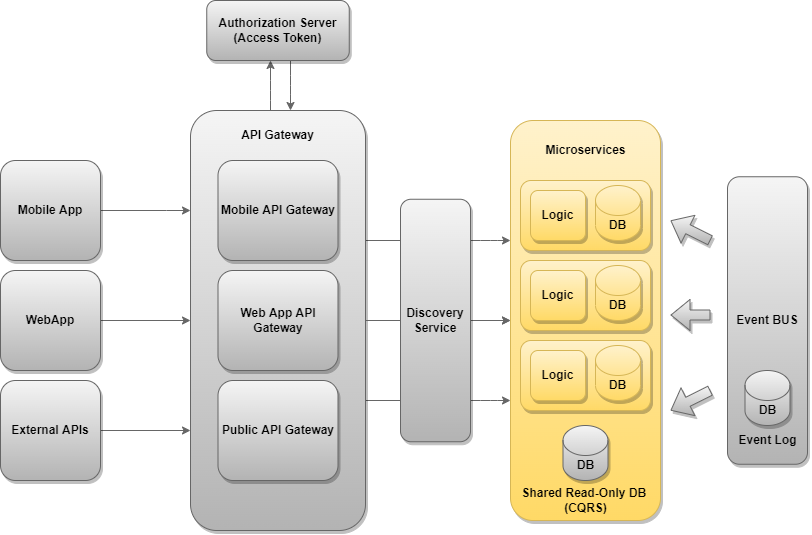
\includegraphics[scale=0.4]{Images/Impl, Integr & Test/Integration Plan - Step 1.png}
	\caption{\label{fig:integration_plan_step_1}Integration - Step 1}
\end{figure}

After this, the Event BUS is the next thing to add, together with the Shared Read-Only DB. The Event BUS will implement all the design patterns related to database communication between microservices, in order to guarantee a correct transmission of information. The Shared Read-Only DB, crucial in the CQRS pattern, will be kept up-to-date by every single microservice.

\begin{figure}[H]
	\centering
    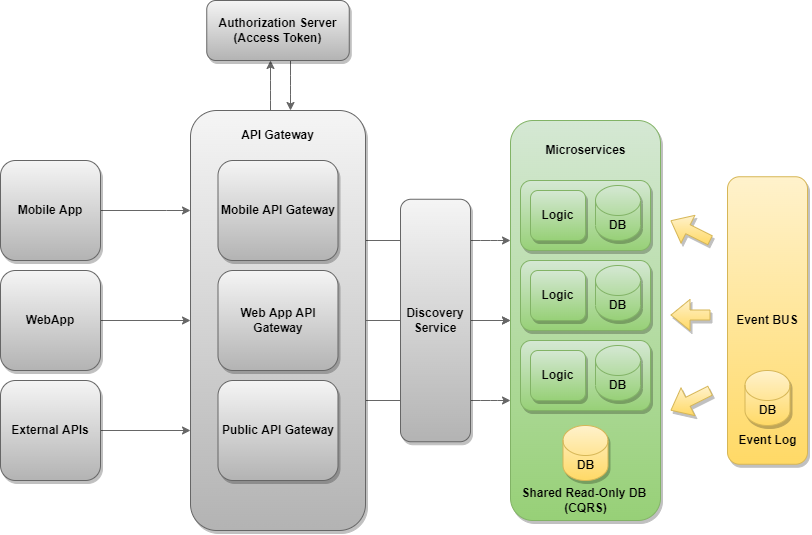
\includegraphics[scale=0.4]{Images/Impl, Integr & Test/Integration Plan - Step 2.png}
	\caption{\label{fig:integration_plan_step_2}Integration - Step 2}
\end{figure}

Now comes the API gateway, that will assure the correct invocation of the methods and functionalities of the microservices, together with the Discovery Service, used for routing the requests to the correct microservice instance and for load balancing.

\begin{figure}[H]
	\centering
    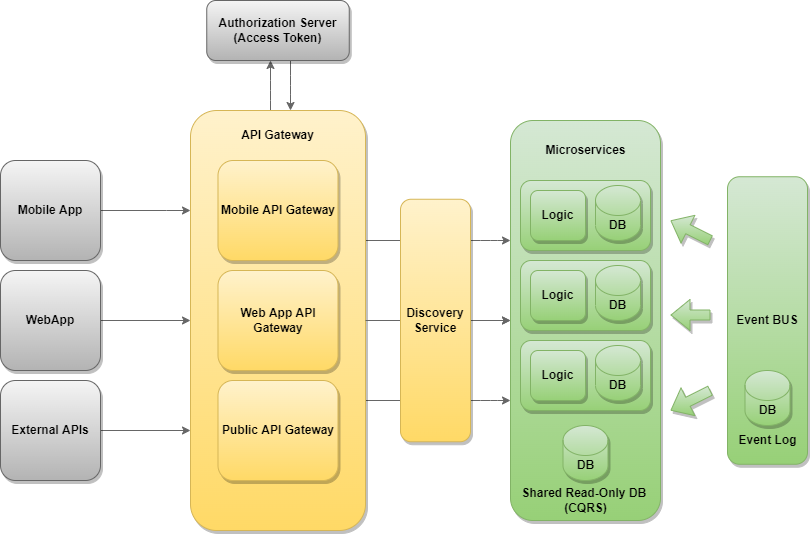
\includegraphics[scale=0.4]{Images/Impl, Integr & Test/Integration Plan - Step 3.png}
	\caption{\label{fig:integration_plan_step_3}Integration - Step 3}
\end{figure}

At this point, it is possible to integrate the authorization server, connected to the API gateway, that will handle all the security aspects, especially those related to authentication and authorization. 

\begin{figure}[H]
	\centering
    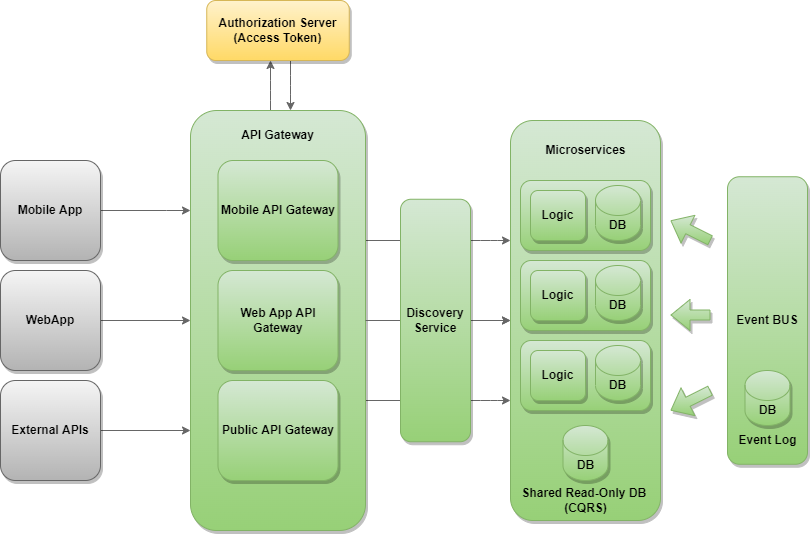
\includegraphics[scale=0.4]{Images/Impl, Integr & Test/Integration Plan - Step 4.png}
	\caption{\label{fig:integration_plan_step_4}Integration - Step 4}
\end{figure}

Then, it is time to integrate the external APIs and Datasets. Since we are assuming them as given and already implemented, we just need to correctly connect them with the rest of the system.

\begin{figure}[H]
	\centering
    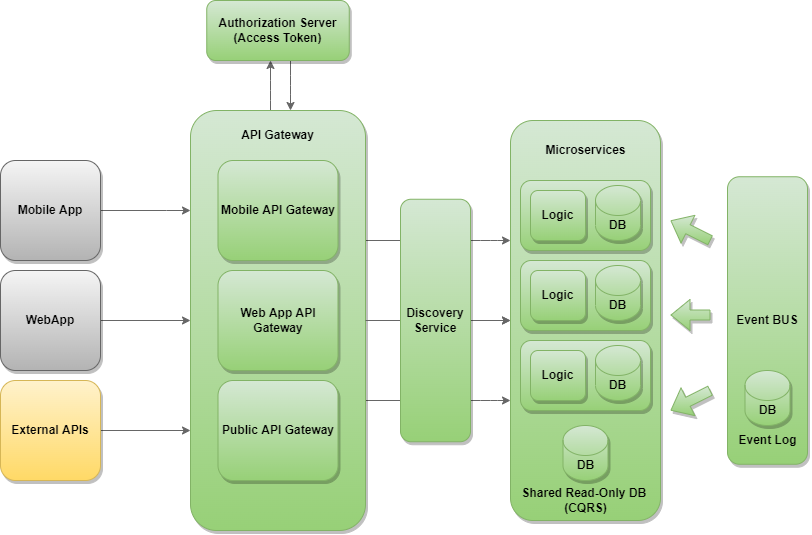
\includegraphics[scale=0.4]{Images/Impl, Integr & Test/Integration Plan - Step 5.png}
	\caption{\label{fig:integration_plan_step_5}Integration - Step 5}
\end{figure}

Finally, it is possible to integrate the mobile application module and the web application module, together with the web browser, that will handle the user-side aspects of the S2B.

\begin{figure}[H]
	\centering
    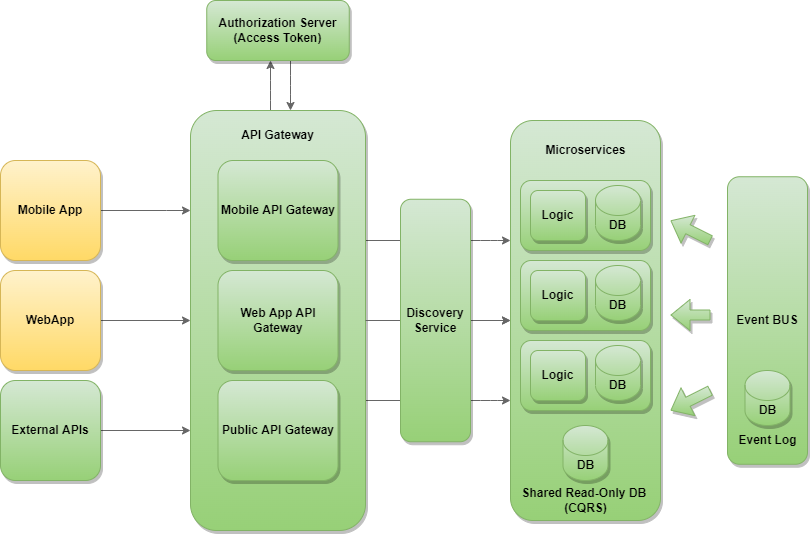
\includegraphics[scale=0.4]{Images/Impl, Integr & Test/Integration Plan - Step 6.png}
	\caption{\label{fig:integration_plan_step_6}Integration - Step 6}
\end{figure}


% ############ 5.3) TEST PLAN ########################
\subsubsection{Test plan}
\label{sec:test_plan}

% ############ 5.3) TEST PLAN ########################

bla bla bla

% ############ 5.4) API TESTING (?) ########################
\subsubsection{API testing}
\label{sec:api_testing}

% ############ 5.4) API TESTING (?) ########################

bla bla bla

%------------------------------------------------------------------------------------------------------------------------------------------------
\clearpage
{\color{Blue}{\section{\label{sect:effort}Effort Spent}}}

In this section we provide detailed information about how much effort each group member spent in working at this document. Further information about commits and updates is stored in the project \href{https://github.com/MarcoRomanini/GoriRomaniniWatanabe}{GitHub} repo. Furthermore also part of the Design Document effort is noted in the table below. 


\begin{center}
    \setlength\arrayrulewidth{1pt}
    \rowcolors{2}{myblue!25}{white}
    \begin{longtable}{llccc}
        
        \hline
        \rowcolor{myblue}\color{white}Date & \color{white}Description & \color{white}Gori & \color{white}Romanini & \color{white}Watanabe \\
        \hline
        29/10	&	World and Machine phenomena	&	2	&	2	&	2	\\
        \hline
        31/10	&	UML	&	1	&	1	&	1	\\
        \hline
        10/11	&	Goals, Domain assumptions, Requirements	&	3	&	3	&	3	\\
        \hline
        17/11	&	UML	&	4	&	4	&	4	\\
        \hline
        19/11	&	Functional requirements	&	4	&	4	&	4	\\
        \hline
        22/11	&	Actors	&		&	2	&		\\
        	&	Perspective (interfaces)	&	3	&		&		\\
        	&	Interface requirements	&		&		&	3	\\
        \hline
        24/11	&	Perspective (interfaces)	&	3	&		&		\\
        	&	Software system attributes	&		&	3	&		\\
        	&	Interface requirements	&		&		&	4	\\
        	&	Functional requirements	&	1	&	1	&		\\
        \hline
        26/11	&	Performance requirements	&		&	2	&		\\
        	&	Design constraints	&	3	&		&		\\
        	&	Functional requirements	&		&	2	&		\\
        	&	Product functions	&		&		&	4	\\
        	&	UI description	&		&		&	1	\\
        \hline
        29/11	&	Functional requirements	&		&	3	&		\\
        	&	farmer bpmn	&	3	&		&		\\
        \hline
        1/12	&	Alloy code	&		&	4	&		\\
        	&	farmer sequence diagram	&	3	&		&		\\
        	&	Users section introduction	&	1	&		&		\\
        \hline
        3/12	&	Goals, Domain assumptions, Requirements	&		&	1	&		\\
        	&	Alloy code	&		&	1,5	&		\\
        	&	Farmers goals mapping	&	2	&		&		\\
        \hline
        06/12	&	Alloy code	&		&	5	&		\\
        	&	UML	&		&	0,5	&		\\
        	&	UI description	&		&		&	3	\\
        	&	Goals, Domain assumptions, Requirements	&		&		&	4	\\
        	&	Introduction	&	6	&		&		\\
        \hline
        07/12	&	Functional Requirements (sequence diagrams, scenarios)	&		&	5	&		\\
        	&	UI design	&		&		&	5	\\
        	&	Sequence diagram	&		&		&	2	\\
        	&	bibliography	&	3	&		&		\\
        	&	latex edits, acronyms table	&	3	&		&		\\
        \hline
        10/12	&	UML diagram	&		&	1,5	&	1,5	\\
        	&	Functional Requirements (use cases)	&		&	1	&		\\
        	&	Product functions	&		&	2	&		\\
        	&	Farmers scenarios	&	3	&		&		\\
        	&	Use case diagram	&		&		&	2	\\
        	&	Policy maker scenarios	&		&		&	2	\\
        \hline
        13/12	&	Architecture Structure (Microservices)	&		&	3	&	3	\\
        \hline
        15/12	&	BPMN	&		&	0,5	&		\\
        	&	Alloy code	&		&	1	&		\\
        	&	Architecture Structure (Microservices)	&		&	1,5	&		\\
        	&	UML diagram	&		&		&	0,5	\\
        	&	BPMN	&		&		&	1	\\
        	&	Goals, Domain assumptions, Requirements	&		&		&	1	\\
        	&	Use case	&		&		&	1	\\
        	&	transcribed goals and requirements	&	1.5	&		&		\\
     	    &	transcribed domain assumptions and traceability matrix   	&	1.5	&		&		\\
        \hline
        17/12	&	UML description	&		&	1,5	&		\\
        	&	Added Alloy code with assertion	&	2	&		&		\\
        \hline
        20/12	&	Functional requirements	&		&	3,5	&		\\
        	&	Architecture Structure (Microservices)	&	1,5	&	1,5	&	1,5	\\
        	&	Alloy code	&		&	1	&		\\
        	&	UML diagram	&		&		&	1	\\
        	&	Goals, Domain assumptions, Requirements	&		&		&	1	\\
        	&	Sequence diagram	&		&		&	2	\\
        	&	Use cases	&		&		&	0,5	\\
        	&	Alloy code transcription	&	2	&		&		\\
        	&	Sequence diagram update	&	1	&		&		\\
        	&	Introduction revise	&	0.5	&		&		\\
        \hline
        20/12 & Effort table & 0.5 &    & \\
         & Whole document review & 7 & 7 & 7\\
        \hline
        
        \rowcolor{white}\caption{\label{tab:effort}Table of efforts.}
        
    \end{longtable}
\end{center}


\end{document}
